% =====================================================================
%  EPIC 2026 — 5th Engineering Physics International Conference
%  FULL PAPER (Stage 2) — DRAFT
%
%  Template  : AIPCP_Article_Template_Sept1_2023.docx
%  Pedoman   : EPIC2026_Author_Guidelines.pdf, bagian 3
%  Tenggat   : Full Paper 20 Sep 2026 | Revisi 15 Okt 2026 | Konferensi 24 Okt 2026
%
%  STATUS: DRAFT KERANGKA. Seluruh angka masih placeholder \val{...} berwarna
%  merah. Sumber angka yang SAH hanya:
%      swarm_ws/results/s2_gamma_20260830_191340/{summary.json,analysis_table.txt}
%  JANGAN pakai results/regions_20260830_130140/ — itu sweep SEBELUM perbaikan
%  gamma (commit 526b0d6), di situ H-inf masih identik dengan LQR.
%
%  Kompilasi: pdflatex -> bibtex -> pdflatex -> pdflatex
%             (atau cukup: latexmk -pdf main.tex)
%
%  Gambar : semua di figures/ ; Pustaka: references.bib (style aipnum4-1)
% =====================================================================
\synctex=1
\documentclass[10pt,letterpaper]{article}

% ---------- Halaman: margin AIP, TIDAK BOLEH diubah ----------
\usepackage[letterpaper,top=1in,bottom=1.18in,left=1in,right=1in]{geometry}

% ---------- Times New Roman untuk teks dan matematika ----------
% amsmath/amssymb WAJIB dimuat sebelum newtxmath: kalau dibalik, keduanya
% sama-sama mendefinisikan \Bbbk dan kompilasi gagal total.
\usepackage[T1]{fontenc}
\usepackage[utf8]{inputenc}
\usepackage{amsmath,amssymb}
\usepackage{newtxtext,newtxmath}

\usepackage{setspace}
\singlespacing                 % AIP: spasi 1.0 di seluruh dokumen

\usepackage{graphicx}
\usepackage{booktabs}          % rule atas/bawah/header saja, tanpa garis vertikal
\usepackage{array}
\usepackage{caption}
\usepackage{changepage}        % indent abstrak 0.2 inci
\usepackage{xcolor}
% TikZ dipakai untuk ilustrasi konsep (Gambar boustrophedon, barrier, FT-CC).
% Gambar arsitektur sendiri berupa JPG, jadi tikz sempat dilepas; dipasang lagi.
\usepackage{tikz}
\usetikzlibrary{arrows.meta,positioning,patterns,patterns.meta,calc,decorations.pathreplacing}
\usepackage{enumitem}
\usepackage[hidelinks]{hyperref}

% ---------- Warna lapisan, disamakan dengan figures/architecture.jpg ----------
\definecolor{layerhigh}{HTML}{2E86AB}
\definecolor{layermid}{HTML}{A23B72}
\definecolor{layerlow}{HTML}{F18F01}
\definecolor{layersim}{HTML}{1B998B}

% ---------- AIP: tanpa header, footer, maupun nomor halaman ----------
\pagestyle{empty}

% ---------- Float: dokumen ini padat gambar/tabel ----------
% Dengan nilai bawaan LaTeX menolak menaruh >2 float per halaman dan menyisakan
% halaman setengah kosong; naskah jadi 10 halaman padahal isinya cukup 7.
\setcounter{topnumber}{3}
\setcounter{bottomnumber}{2}
\setcounter{totalnumber}{4}
\renewcommand{\topfraction}{0.92}
\renewcommand{\bottomfraction}{0.75}
\renewcommand{\textfraction}{0.07}
\renewcommand{\floatpagefraction}{0.80}

% ---------- Paragraf: indent baris pertama 0.2", rata kiri-kanan ----------
\setlength{\parindent}{0.2in}
\setlength{\parskip}{0pt}

% ---------- Jarak sekitar persamaan display ----------
% Bawaan LaTeX boros; dokumen ini punya 39 persamaan bernomor.
\setlength{\abovedisplayskip}{6pt}
\setlength{\belowdisplayskip}{6pt}
\setlength{\abovedisplayshortskip}{3pt}
\setlength{\belowdisplayshortskip}{3pt}

% ---------- Caption 9 pt, centered ----------
% Gambar: label "FIGURE n." bold, caption DI BAWAH gambar.
% Tabel : label "TABLE n." bold, caption DI ATAS tabel.
\DeclareCaptionLabelFormat{aipfigure}{\textbf{FIGURE #2.}}
\DeclareCaptionLabelFormat{aiptable}{\textbf{TABLE #2.}}
\captionsetup[figure]{labelformat=aipfigure,labelsep=space,font=small,
    justification=centering,singlelinecheck=true,skip=6pt}
\captionsetup[table]{labelformat=aiptable,labelsep=space,font=small,
    justification=centering,singlelinecheck=true,skip=4pt}

% ---------- Heading AIP ----------
% Level 1: 12 pt bold ALL CAPS centered
% Level 2: 12 pt bold centered, Initial Caps
% Level 3: 10 pt italic centered, Initial Caps
\newcommand{\headingone}[1]{%
    \par\vspace{9pt}%
    {\centering\fontsize{12}{14}\selectfont\bfseries\MakeUppercase{#1}\par}%
    \vspace{4pt}\noindent\ignorespaces}
\newcommand{\headingtwo}[1]{%
    \par\vspace{7pt}%
    {\centering\fontsize{12}{14}\selectfont\bfseries #1\par}%
    \vspace{3pt}\noindent\ignorespaces}
\newcommand{\headingthree}[1]{%
    \par\vspace{6pt}%
    {\centering\fontsize{10}{12}\selectfont\itshape #1\par}%
    \vspace{2pt}\noindent\ignorespaces}

% ---------- Penanda draft ----------
% \val{} = slot angka yang belum diisi dari CSV. Sengaja mencolok.
% \TODO{} = catatan kerja, harus nol sebelum submit.
\newcommand{\val}[1]{\textcolor{red}{\textbf{#1}}}
\newcommand{\TODO}[1]{\textcolor{red}{\textbf{[TODO: #1]}}}

% ---------- Sitasi & bibliografi bergaya AIP ----------
% aipnum4-1.bst adalah style AIP asli. Ia dirancang untuk REVTeX, jadi di kelas
% article beberapa makro yang dipancarkannya belum terdefinisi; shim di bawah
% mendefinisikannya sebagai no-op supaya bisa dipakai tanpa REVTeX.
\usepackage[numbers,sort&compress]{natbib}
\providecommand{\bibinfo}[2]{#2}
\providecommand{\bibnamefont}[1]{#1}
\providecommand{\bibfnamefont}[1]{#1}
\providecommand{\citenamefont}[1]{#1}
\providecommand{\natexlab}[1]{#1}
\providecommand{\eprint}[2][]{\url{#2}}
\providecommand{\doibase}{https://doi.org/}
\providecommand{\urlprefix}{}
\providecommand{\Doi}[1]{\href{\doibase#1}{#1}}
\providecommand{\BibitemOpen}{}
\providecommand{\BibitemShut}[1]{}
\providecommand{\bibAnnote}[2]{}
\providecommand{\selectlanguage}[1]{}
% Pedoman AIP bagian 4: penanda daftar pustaka "1." (angka + titik), sedangkan
% sitasi di dalam teks tetap kurung siku [1], [2,3]. natbib memberi [1] pada
% keduanya, jadi penanda daftarnya ditimpa di sini.
\makeatletter
\renewcommand{\@biblabel}[1]{#1.}
\makeatother
% Rujukan AIP dicetak [1], [2,3] — natbib numbers sudah begitu.
\newcommand{\cit}[1]{\cite{#1}}
\newcommand{\citt}[2]{\cite{#1,#2}}



\begin{document}

% =====================================================================
%  JUDUL / PENULIS / AFILIASI / EMAIL — persis dari abstrak yang diterima
% =====================================================================
\begin{center}
    {\fontsize{18}{22}\selectfont\bfseries
        Fault-Tolerant Swarm Quadrotor Control for Non-Convex\\
        Geodetic Mapping\par}

    \vspace{2.0ex}

    {\fontsize{14}{17}\selectfont
        Izma Alhazmi Herdian\textsuperscript{1,2,a)},
        Sulthan Naufal Affan\textsuperscript{1,b)}, and
        Estiyanti Ekawati\textsuperscript{1,2,c)}\par}

    \vspace{1.5ex}

    {\fontsize{10}{12}\selectfont\itshape
        \textsuperscript{1}Engineering Physics Department, Institut Teknologi Bandung,
        Bandung 40132, Indonesia\\
        \textsuperscript{2}Center for Instrumentation Technology and Automation,
        Institut Teknologi Bandung, Bandung 40132, Indonesia\par}

    \vspace{1.5ex}

    {\fontsize{10}{12}\selectfont\itshape
        \textsuperscript{a)}Corresponding author: izmaherdian@gmail.com\\
        \textsuperscript{b)}sulthannaufal96@gmail.com\\
        \textsuperscript{c)}esti@itb.ac.id\par}
\end{center}

\vspace{1.5ex}

\begin{adjustwidth}{0.2in}{0.2in}
    {\fontsize{9}{11}\selectfont
        \noindent\textbf{Abstract.} This paper presents a three-layer control architecture
        for autonomous geodetic mapping of non-convex regions by a quadrotor swarm. The
        high-level layer partitions the region by centroidal Voronoi tessellation, generates
        a polygon-aware boustrophedon sweep for each cell, and redistributes coverage through
        Fault-Tolerant Cooperative Coverage (FT-CC) on agent loss. The mid-level layer
        enforces safety through a control barrier function quadratic program (CBF-QP) solved
        once per agent per control tick, with a class-$\mathcal{K}$ function derived from the
        vehicle tilt limit and dead time. The low-level layer is a cascaded PID whose gains
        are synthesised either from the algebraic Riccati equation (LQR) or from the
        $H_\infty$ Riccati equation. The architecture is validated in ROS~2 and Gazebo over three
        non-convex regions and two controllers along a load ladder that adds one stressor at
        a time: nominal, turbulence, turbulence with obstacles, and turbulence with obstacles
        and sequential agent loss. Coverage held at \val{XX.X--XX.X\%} with zero inter-agent
        collisions throughout; $H_\infty$ reduced cross-track RMS error by \val{XX\%} under
        turbulence at \val{X.X$\times$} the control effort, and FT-CC recovered coverage to
        within \val{X.X} percentage points of the no-failure condition after losing two of
        seven agents.
        \par}
\end{adjustwidth}

% =====================================================================
\headingone{Introduction}

Swarm quadrotor systems support autonomous geodetic mapping in disaster response,
precision agriculture, environmental surveillance, and infrastructure inspection.
Partitioning a territory among several agents converts a sequential survey into a
parallel one, but doing so requires region partitioning, robust flight control under
disturbance, and continued operation after agent failure.

Four gaps persist across the literature reviewed in the next section. First, most
coverage algorithms assume a \emph{convex} operational region
\citt{papatheodorouCooperativeVisual2017}{huRoutePlanning2021}, whereas survey areas are
non-convex by construction. Second, end-to-end pipelines from partitioning down to rotor
control are scarce \cit{huRoutePlanning2021}: planning and execution are normally
developed and reported separately, hiding the integration mismatches that appear only
when they are connected. Third, fault tolerance under actuator or communication failure
is underexplored \cit{okeeffeAnticipatingDegradation2025}, although the probability that
\emph{some} agent fails grows with swarm size. Fourth, validation is predominantly
carried out on kinematic point-mass models rather than full quadrotor dynamics
\cit{belkheiriLinearizationControl2012}; path lengths, mission durations, and safety
margins obtained that way are measured on a vehicle whose tilt limit, motor lag, and
dead time do not exist.

This paper contributes: (i) a polygon-aware coverage planner whose extremal sweep rows
follow the cell boundary, eliminating the unswept wedges a fixed-pitch sweep leaves at
tapered corners; (ii) a CBF-QP that folds static obstacles, moving obstacles, arena
walls, and reciprocal inter-agent spacing into one quadratic program with an
actuator-consistent class-$\mathcal{K}$ function derived from the identified closed-loop
plant; (iii) a like-for-like comparison of LQR and $H_\infty$ gain synthesis on an
identical cascade, including the selection procedure for the attenuation bound $\gamma$;
and (iv) an evaluation on full six-degree-of-freedom dynamics over three non-convex
regions, under nominal, turbulent, and agent-failure conditions.

% =====================================================================
\headingone{Related Work}

\headingtwo{Coverage Control and Region Partitioning}

Coverage control by centroidal Voronoi tessellation was established by Cort\'es
\emph{et al.} \cit{cortesCoverageControl2004}, who showed that a Lloyd descent
\cit{lloydLeastSquaresQuantization1982} on the Voronoi centroids
\cit{duCentroidalVoronoiTessellations1999} converges to a locally optimal sensor
configuration. The formulation is elegant but assumes a convex domain: the centroid of a
non-convex cell may fall outside the cell, and the geodesic and Euclidean metrics
diverge. Extensions to non-convex domains take three broad routes --- diffeomorphic
mapping to a convex proxy, geodesic distance computation, and local navigation around
obstacles. Breitenmoser \emph{et al.} \cit{breitenmoserVoronoiCoverage2010} combine Lloyd
descent with the TangentBug local planner and prove convergence in non-convex polygons;
Lee and Lee \cit{leeAdaptiveCentroidalVoronoi2024} instead add agent dropout and
reinsertion to escape the local minima that non-convex domains introduce; Cao \emph{et
    al.} \cit{caoDistributedWeightedCoverage2023} use buffered Voronoi cells to embed
collision margins directly in the partition. The present work follows the third route in
spirit but keeps the partition purely geometric: cells are clipped against the survey
polygon itself, and safety margins are enforced downstream by the barrier layer rather
than baked into the cell boundaries.

\headingtwo{Coverage Path Planning}

Given a cell, the sweep itself is a coverage path planning problem, surveyed by Choset
\cit{chosetCoverageSurvey2001} and later by Galceran and Carreras
\cit{galceranCoveragePathPlanning2013}. Boustrophedon cellular decomposition
\cit{chosetBoustrophedonDecomposition1998} remains the standard: the free space is
decomposed into cells sweepable by simple back-and-forth motions. Most implementations
sweep with a fixed pitch and a fixed direction, which is exact for rectangular cells and
leaves systematic gaps at tapered corners --- precisely the geometry that non-convex
Voronoi partitioning produces most often. Route optimisation in this family typically
targets the number of turns and the total path length
\cit{huRoutePlanning2021,galceranCoveragePathPlanning2013}, and is normally evaluated on
kinematic agents, so the turn cost is a count rather than a dynamic penalty.

\headingtwo{Reciprocal Collision Avoidance and Safety Filters}

For multi-agent deconfliction, control barrier functions provide forward invariance of a
designated safe set through a single inequality constraint on the control
\cit{amesControlBarrierFunction2017,amesControlBarrierFunctions2019}. Wang \emph{et al.}
\cit{wangSafetyBarrierCertificates2017} extend this to reciprocal multi-robot safety with
safety barrier certificates, and Zhou \emph{et al.} \cit{zhouBufferedVoronoiCells2017}
achieve a comparable guarantee geometrically through buffered Voronoi cells. In the
canonical formulation the class-$\mathcal{K}$ function is linear, $\alpha(h)=\gamma h$,
with $\gamma$ chosen by tuning. That choice is adequate when the actuator can deliver the
implied deceleration, but a quadrotor's lateral acceleration is bounded by its tilt limit
and its command path carries dead time, so the admissible approach speed near contact is
dictated by braking capability rather than by a tuning constant. The barrier used here,
Eq.~\eqref{eq:e14}, is derived from that braking capability directly.

\headingtwo{Fault Tolerance in Swarms}

Fault tolerance in robot swarms is predominantly reactive: a failure is detected, then the
task is redistributed. O'Keeffe \cit{okeeffeAnticipatingDegradation2025} argues for the
predictive alternative, resolving degradation before it becomes failure, and reports
comparable or better performance than a reactive baseline. The mechanism used here is
reactive by design --- heartbeat timeout, compound-polygon merge, helper reallocation ---
because the failures of interest are abrupt losses rather than gradual degradation, but
the two are complementary rather than exclusive.

% =====================================================================
\headingone{Methodology}

\headingtwo{System Architecture}

Figure~\ref{fig:arch} shows the three layers. The high-level layer consumes the survey
polygon and initial poses and emits waypoints. The mid-level layer maps the desired
velocity to a certified-safe commanded velocity. The low-level layer tracks the resulting
reference and outputs rotor speeds. Odometry closes the loop at every level. The state
machine never writes a velocity command directly: it writes a desired velocity that is
filtered through the QP in a single function, so the avoidance layer is separable from
the planner.
% Diagram arsitektur: docs/Diagram-Swarm-Quadrotor-Mapping-v1.jpg, disalin ke
% figures/architecture.jpg. Versi v1 sudah memuat label yang benar (CBF-QP
% Solver; Gazebo Harmonic Physics tanpa PX4 SITL), jadi tidak perlu koreksi.
% CATATAN: teks "Coverage >= 95%" tercetak di dalam JPG dan TIDAK bisa diubah
% dari LaTeX — kalau angka final sudah masuk, perbarui gambarnya di drawio.
\begin{figure}[tbp]
    \centering
    
\includegraphics[width=\textwidth]{figures/architecture.jpg}
    \caption{Three-layer control architecture for resilient swarm geodetic mapping. Each
        agent runs the full stack locally and communicates over a peer-to-peer DDS mesh.
        Command signals flow downward, state feedback upward, and heartbeat loss triggers
        re-partitioning in the FT-CC module.}
    \label{fig:arch}
\end{figure}

\headingtwo{High-Level Layer: Coverage Planning and Resilience}

\headingthree{Centroidal Voronoi Partitioning}

Let $\Omega\subset\mathbb{R}^2$ be the survey polygon, not assumed convex, and
$\mathbf{p}_i$ the seed of agent $i$, $i=1,\dots,N$. The Voronoi cell of agent $i$ is

\begin{equation}
    \label{eq:e1}
    V_i=\bigl\{\mathbf{p}\in\Omega \;\bigm|\; \|\mathbf{p}-\mathbf{p}_i\|\le
    \|\mathbf{p}-\mathbf{p}_j\|,\ \forall j\neq i\bigr\},
\end{equation}

obtained by successive Sutherland--Hodgman clipping of $\Omega$ against the perpendicular
bisector $H_{ij}$ of each pair,

\begin{equation}
    \label{eq:e2}
    H_{ij}=\Bigl\{\mathbf{p} \;\Bigm|\;
    (\mathbf{p}_j-\mathbf{p}_i)^{\!\top}
    \Bigl(\mathbf{p}-\tfrac{\mathbf{p}_i+\mathbf{p}_j}{2}\Bigr)\le 0\Bigr\},
    \qquad V_i=\Omega\cap\bigcap_{j\neq i}H_{ij}.
\end{equation}

Cells are equalised by Lloyd iteration \cit{lloydLeastSquaresQuantization1982}, moving
each seed to the area centroid of its own cell, which is the discrete descent underlying
centroidal Voronoi coverage control
\citt{cortesCoverageControl2004}{duCentroidalVoronoiTessellations1999},

\begin{equation}
    \label{eq:e3}
    \mathbf{p}_i^{(k+1)}=\frac{1}{|V_i^{(k)}|}\iint_{V_i^{(k)}}\mathbf{p}\,\mathrm{d}A,
    \qquad
    |V_i^{(k)}|=\iint_{V_i^{(k)}}\mathrm{d}A,
\end{equation}

run for $12$ iterations. Clipping acts on the polygon itself rather than a bounding box,
so concave boundaries and interior exclusions need no diffeomorphism, geodesic metric, or
auxiliary markers \citt{leeAdaptiveCentroidalVoronoi2024}{breitenmoserVoronoiCoverage2010}. Each cell is then eroded by a margin
$\delta_c=0.35$~m before planning \cit{caoDistributedWeightedCoverage2023}.

\headingthree{Sensing Model and Coverage Semantics}

The sweep pitch is not free: it is fixed by the mapping payload. For a downward-looking
camera of focal length $f$, pixel pitch $p$, and sensor width $s_w$, flown at altitude
$h_a$, the ground sampling distance and the across-track swath are

\begin{equation}
    \mathrm{GSD}=\frac{h_a\,p}{f},
    \qquad
    w=\frac{h_a\,s_w}{f}=2h_a\tan\frac{\Phi}{2},
    \label{eq:gsd}
\end{equation}

with $\Phi$ the across-track field of view. Photogrammetric reconstruction requires a side
overlap $o_s$ between adjacent strips, which bounds the pitch and hence the effective
sensing radius used by the planner,

\begin{equation}
    \Delta y\le w\,(1-o_s),
    \qquad
    r_s=\tfrac{1}{2}w\,,
    \label{eq:pitch}
\end{equation}

so that a cell is fully mapped, not merely overflown. Coverage in this paper is evaluated
against the disc model of Eq.~\eqref{eq:pitch}: a grid cell counts as observed once its
centre falls within $r_s$ of some agent. This is a geometric abstraction of the payload,
and it is the same abstraction used by the coverage-control literature
\cit{cortesCoverageControl2004}. It deliberately does not model radiometric quality,
feature matching, or bundle-adjustment residuals, so the reported $\eta$ quantifies
\emph{area coverage at the required GSD}, not final map accuracy; the distinction is
revisited among the limitations.

\headingthree{Polygon-Aware Boustrophedon Sweep}

Each cell is swept by boustrophedon decomposition
\citt{chosetBoustrophedonDecomposition1998}{chosetCoverageSurvey2001}. For cell $V_i$
with vertical extent $[y_{\min},y_{\max}]$ and sweep pitch $\Delta y$, the scanline set
is $\mathcal{Y}_i=\{y_{\min}+k\Delta y\}$, and each scanline yields the
intervals

\begin{equation}
    \label{eq:e4}
    S_i(y)=\bigl\{[x_{2k-1}(y),\,x_{2k}(y)]\bigr\}_{k=1}^{m(y)},
    \qquad
    \{x_1(y)<\dots<x_{2m}(y)\}=\partial V_i\cap\{\,\cdot\,,y\},
\end{equation}

where $m(y)>1$ for a concave cell. A fixed-pitch horizontal sweep leaves an unswept wedge
between the last scanline and the boundary at any tapered corner. The planner therefore
replaces the extremal rows by the cell's own boundary chains $\mathcal{C}^-_i$ (bottom) and
$\mathcal{C}^+_i$ (top), keeping interior rows horizontal, giving the flat waypoint list

\begin{equation}
    \label{eq:e5}
    \mathcal{W}_i=\mathcal{C}^-_i \;\cup\!\!
    \bigcup_{y\in\mathcal{Y}_i\setminus\{y_{\min},y_{\max}\}}\!\!\sigma_y\bigl(S_i(y)\bigr)
    \;\cup\; \mathcal{C}^+_i,
\end{equation}

with $\sigma_y$ reversing the traversal direction on alternate rows;
Figure~\ref{fig:wedge} contrasts the two constructions.
% ---------------------------------------------------------------------
% Ilustrasi konsep baji tak tersapu + rantai tepi. Ditambah anotasi pitch,
% jejak sensor r_s, dan aturan penggabungan verteks. Skematik.
% ---------------------------------------------------------------------
\begin{figure}[tbp]
    \centering
    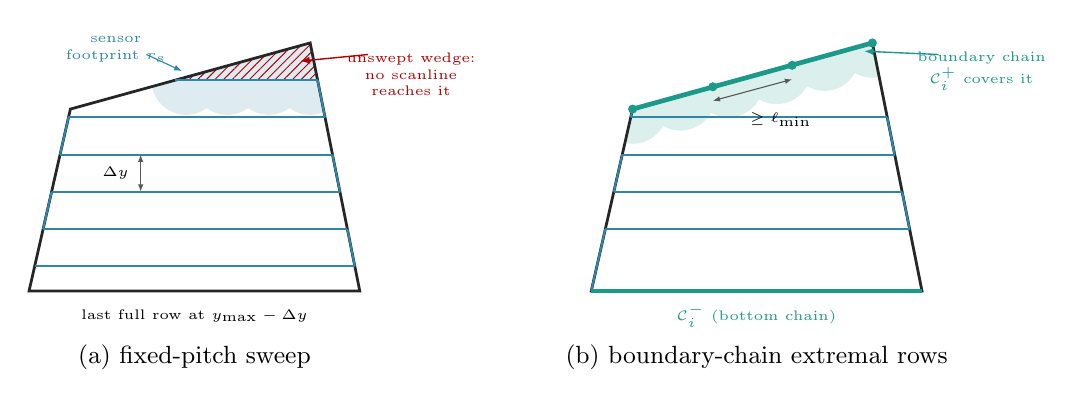
\begin{tikzpicture}[
            scale=1.05,
            every node/.style={font=\scriptsize},
            cellb/.style={draw=black!85, line width=1.0pt},
            sweep/.style={draw=layerhigh, line width=0.75pt},
            chain/.style={draw=layersim, line width=1.7pt},
            lbl/.style={font=\tiny},
            panel/.style={font=\small}
        ]
        \def\Cell{(0,0) -- (4,0) -- (3.4,3.0) -- (0.5,2.2) -- cycle}

        % ================= (a) sapuan pitch tetap =========================
        \begin{scope}
            % jejak sensor pada baris terakhir: menunjukkan baji tetap di luar jangkauan
            \begin{scope}
                \clip \Cell;
                \foreach \x in {1.9,2.4,2.9,3.4}
                \fill[layerhigh!16] (\x,2.55) circle (0.42);
            \end{scope}

            \fill[pattern={Lines[angle=45,distance=2.2pt,line width=0.35pt]},
                pattern color=red!70!black]
            (1.769,2.55) -- (3.49,2.55) -- (3.4,3.0) -- cycle;
            \draw[red!70!black, line width=0.55pt]
            (1.769,2.55) -- (3.49,2.55) -- (3.4,3.0) -- cycle;

            \draw[cellb] \Cell;
            \foreach \y/\xa/\xb in {0.30/0.068/3.94, 0.75/0.170/3.85, 1.20/0.273/3.76,
                    1.65/0.375/3.67, 2.10/0.477/3.58, 2.55/1.769/3.49}
            \draw[sweep] (\xa,\y) -- (\xb,\y);
            \draw[sweep] (3.94,0.30) -- (3.85,0.75);
            \draw[sweep] (0.170,0.75) -- (0.273,1.20);
            \draw[sweep] (3.76,1.20) -- (3.67,1.65);
            \draw[sweep] (0.375,1.65) -- (0.477,2.10);
            \draw[sweep] (3.58,2.10) -- (3.49,2.55);

            % anotasi pitch
            \draw[{Latex[scale=0.55]}-{Latex[scale=0.55]}, black!65, line width=0.4pt]
            (1.35,1.20) -- (1.35,1.65);
            \node[lbl, left] at (1.32,1.43) {$\Delta y$};

            % jejak sensor
            \node[lbl, text=layerhigh, align=center] at (1.05,2.92) {sensor\\footprint $r_s$};
            \draw[-{Latex[scale=0.6]}, layerhigh, line width=0.4pt]
            (1.42,2.86) -- (1.85,2.66);

            \node[lbl, text=red!70!black, align=center] at (4.62,2.62)
            {unswept wedge:\\no scanline\\reaches it};
            \draw[-{Latex[scale=0.65]}, red!70!black, line width=0.5pt]
            (4.10,2.86) -- (3.28,2.78);

            \node[lbl] at (2.0,-0.30) {last full row at $y_{\max}-\Delta y$};
            \node[panel] at (2,-0.80) {(a) fixed-pitch sweep};
        \end{scope}

        % ================= (b) baris rantai-tepi ==========================
        \begin{scope}[shift={(6.8,0)}]
            \begin{scope}
                \clip \Cell;
                \foreach \t in {0,0.2,...,1.01}
                \fill[layersim!16]
                ({0.5+2.9*\t},{2.2+0.8*\t}) circle (0.42);
            \end{scope}

            \draw[cellb] \Cell;
            \foreach \y/\xa/\xb in {0.75/0.170/3.85, 1.20/0.273/3.76,
                    1.65/0.375/3.67, 2.10/0.477/3.58}
            \draw[sweep] (\xa,\y) -- (\xb,\y);
            \draw[sweep] (3.85,0.75) -- (3.76,1.20);
            \draw[sweep] (0.273,1.20) -- (0.375,1.65);
            \draw[sweep] (3.67,1.65) -- (3.58,2.10);

            \draw[chain] (0,0) -- (4,0);
            \draw[chain] (0.5,2.2) -- (3.4,3.0);
            \draw[sweep] (0.477,2.10) -- (0.5,2.2);
            \draw[sweep] (0.170,0.75) -- (0,0);

            % verteks rantai + aturan penggabungan
            \foreach \p in {(0.5,2.2),(1.47,2.47),(2.43,2.73),(3.4,3.0)}
            \fill[layersim] \p circle (0.055);
            \draw[{Latex[scale=0.55]}-{Latex[scale=0.55]}, black!65, line width=0.4pt]
            (1.47,2.30) -- (2.43,2.56);
            \node[lbl, below right] at (1.80,2.28) {$\ge\ell_{\min}$};

            \node[lbl, text=layersim, align=center] at (4.72,2.66)
            {boundary chain\\$\mathcal{C}^+_i$ covers it};
            \draw[-{Latex[scale=0.65]}, layersim, line width=0.5pt]
            (4.20,2.86) -- (3.30,2.90);
            \node[lbl, text=layersim] at (2.0,-0.30) {$\mathcal{C}^-_i$ (bottom chain)};

            \node[panel] at (2,-0.80) {(b) boundary-chain extremal rows};
        \end{scope}
    \end{tikzpicture}
    \caption{Why the extremal sweep rows follow the cell boundary, drawn schematically for a
        tapered cell. (a) Horizontal scanlines at a fixed pitch $\Delta y$ stop at the last
        full row; the sensor footprint of radius $r_s$ (shaded) does not reach the wedge
        between that row and the boundary, so the wedge is never mapped, and the defect grows
        with the acuteness of the corner. (b) Replacing the first and last rows by the cell's
        own boundary chains $\mathcal{C}^-_i$ and $\mathcal{C}^+_i$, Eq.~\eqref{eq:e5}, sweeps
        the boundary itself and closes the wedge by construction, while interior rows stay
        horizontal. Chain vertices closer than $\ell_{\min}$ are merged, since a segment
        shorter than the braking distance at cruise speed cannot be decelerated into.}
    \label{fig:wedge}
\end{figure}

 Chain vertices closer
than $\ell_{\min}=0.60$~m are merged: a segment shorter than the braking distance at cruise
speed cannot be decelerated into and appears as end-of-row overshoot, while the sensor
radius $r_s=0.95$~m keeps the merged vertices covered. The entry end of $\mathcal{C}^-_i$ is
selected from the agent's current position.

\headingthree{Obstacle Perception and Replanning}

Obstacle positions are not supplied to the planner. Each mission starts with an
\emph{empty} obstacle map, and the swarm builds it while flying, so the coverage results
reported later are those of a system that had to find the cylinders before it could route
around them.

Every LiDAR return is first screened: hits that fall near another agent or near the arena
wall are discarded, since a neighbouring vehicle subtends an arc indistinguishable from a
cylinder. Surviving returns are clustered by angular continuity, and a circle is fitted to
each cluster by algebraic least squares, giving a detection $(\mathbf{c},r)$. Detections
from all agents are merged into one shared map. A detection is associated with an existing
track when it lies within $d_a=1.20$~m of it, otherwise it opens a new track. A track
becomes \emph{confirmed}, and thus visible to the planner and to the barrier layer, only
after $n_{\min}=4$ sightings,

\begin{equation}
    \mathcal{O}^{\mathrm{known}}(t)=\bigl\{\,\tau \;\bigm|\; n_\tau(t)\ge n_{\min}\,\bigr\},
    \qquad
    \mathbf{c}_\tau \leftarrow \mathbf{c}_\tau+\tfrac{1}{n_\tau+1}\bigl(\mathbf{c}-\mathbf{c}_\tau\bigr),
    \label{eq:percep}
\end{equation}

with the centre and radius kept as running means so that a single noisy frame cannot shift
the map. The confirmation threshold is what keeps edge reflections and missed drone
rejections from populating the map with phantom cylinders; a track whose centre drifts
further than $0.70$~m from its anchor is discarded as a moving object rather than promoted.

When a track is confirmed, the agents whose swept cells its keep-out disc intersects
replan. Only rows \emph{above} the current sweep line are replaced: sweeps run bottom to
top, so re-planning a completed row would sweep it twice. Between the moment an obstacle
enters the sensing range and the moment its track is confirmed, nothing in the plan knows
about it, and safety rests entirely on the barrier layer of the next section, which acts on
the same confirmed set $\mathcal{O}^{\mathrm{known}}$.

Two obstacle sets must therefore be distinguished, and conflating them would invalidate the
results. $\mathcal{O}^{\mathrm{known}}$ is what the system knows; the planner and every
constraint row see only this. The ground-truth table $\mathcal{O}^{\mathrm{true}}$ is used
\emph{only} for scoring --- it defines the coverage denominator and detects collisions ---
because grading an agent against obstacles it has not yet discovered is the entire point of
the exercise. No quantity reported in this paper lets $\mathcal{O}^{\mathrm{true}}$ leak
into a control or planning decision.

\headingthree{Obstacle Routing}

Routing acts on the confirmed set $\mathcal{O}^{\mathrm{known}}$ only. For a confirmed
obstacle $k$ at $\mathbf{o}_k$ with radius $\rho_k$ and keep-out radius
$R^{\mathrm{ko}}=1.30$~m, every scanline interval is \emph{split} rather than trimmed,

\begin{equation}
    \label{eq:e6}
    [x_a,x_b]\;\longmapsto\;
    [x_a,x_b]\setminus\bigl\{x \;\bigm|\; \|(x,y)-\mathbf{o}_k\|<R^{\mathrm{ko}}\bigr\},
\end{equation}

which returns a list, so an obstacle lying mid-row is handled. A final pass over the
assembled list inserts circular detour arcs of radius $R^{\mathrm{ko}}$ subtending at most
$70^\circ$ per chord, then string-pulls points back out subject to
$\|\mathbf{w}-\mathbf{o}_k\|\ge R^{\mathrm{cl}}=1.10$~m. The chord of a $70^\circ$ arc dips
to $R^{\mathrm{ko}}\cos 35^\circ=1.065$~m, still above the physical requirement
$\rho_k+r_d+\delta_s=0.40+0.22+0.25=0.87$~m. Since $R^{\mathrm{ko}}<r_s$, the annulus
around each obstacle is mapped during the detour and avoidance costs no coverage. Obstacle
$k$ is assigned to every agent whose swept cell its keep-out disc \emph{intersects},

\begin{equation}
    \label{eq:e7}
    \mathcal{O}_i=\bigl\{k \;\bigm|\;
    \mathcal{B}(\mathbf{o}_k,R^{\mathrm{ko}})\cap V_i\neq\emptyset\bigr\},
\end{equation}

not to the single agent whose cell contains it; exclusive assignment leaves a neighbour
sweeping through a keep-out zone with no detour planned.

\headingthree{Start-Point Deconfliction}

Each agent has two candidate entries $e_i\in\{0,1\}$, one at each end of $\mathcal{C}^-_i$.
Neighbouring cells can place two entries closer than the hard separation $d_{\mathrm{hard}}$,
after which the second agent can never arrive. All $2^N$ assignments are scored
lexicographically,

\begin{equation}
    \label{eq:e8}
    \mathbf{e}^\star=\arg\max_{\mathbf{e}\in\{0,1\}^N}
    \min\Bigl(\min_{i<j}\|\mathbf{s}_i(e_i)-\mathbf{s}_j(e_j)\|,\;d_{\mathrm{cap}}\Bigr),
    \qquad
    \text{tie-break } \min\sum_{i=1}^{N}\|\mathbf{p}_i-\mathbf{s}_i(e_i)\|,
\end{equation}

with $d_{\mathrm{cap}}=2.5$~m so that separation beyond a comfortable margin is not bought
with further transit.

\headingthree{Fault-Tolerant Cooperative Coverage}

Agent health is tracked by peer-to-peer heartbeat. Agent $k$ is declared dead when
$t-t_k^{\mathrm{hb}}>T_{\mathrm{hb}}$. The map an agent has built is carried on the agent, so
losing the vehicle loses the data: on declaring $k$ dead the coordinator \emph{erases} the
occupancy record over the whole of $V_k$ rather than crediting the part $k$ had already
flown. The recovery region is therefore the union of the complete cells of the dead set,

\begin{equation}
    \label{eq:e9}
    V_{\mathrm{merged}}=\bigcup_{k\in\mathcal{D}}V_k ,
    \qquad
    \mathcal{G}\!\left[V_k\right]\leftarrow\text{unobserved},\ \ \forall k\in\mathcal{D},
\end{equation}

with $\mathcal{G}$ the shared occupancy grid. The erasure is deliberately scoped to the dead
agent's own cell: area already re-swept by a helper during an earlier recovery is retained,
since that data sits on a vehicle still flying. A fresh boustrophedon path is generated over
$V_{\mathrm{merged}}$ by Eq.~\eqref{eq:e5}, and its rows are redistributed to at most three
surviving neighbours, which resume their own cells afterwards. Rows still queued on an agent
that dies while acting as a helper are recaptured and folded into the next merge, so no row
is dropped when a failure lands on a helper. Figure~\ref{fig:ftcc-concept} illustrates the
sequence.

This is the conservative choice, and it costs real flight time: a failure at high mission
progress discards a nearly complete cell. It is also the only sound one, because the
coordinator has no way to recover the observations that went down with the vehicle.

% ---------------------------------------------------------------------
% Ilustrasi konsep FT-CC.
% Prinsip tata letak: TIDAK ADA label mengambang di dekat wilayah — semua
% keterangan simbol dipindah ke satu baris legenda di bawah ketiga panel,
% sehingga panelnya sendiri bersih dan ketiganya sebanding.
% Semantik yang harus benar: saat agen gugur, riwayat coverage SELURUH
% selnya dihapus dan sel itu disapu ulang penuh (lihat Eq. V_merged).
% ---------------------------------------------------------------------
\begin{figure}[tbp]
    \centering
    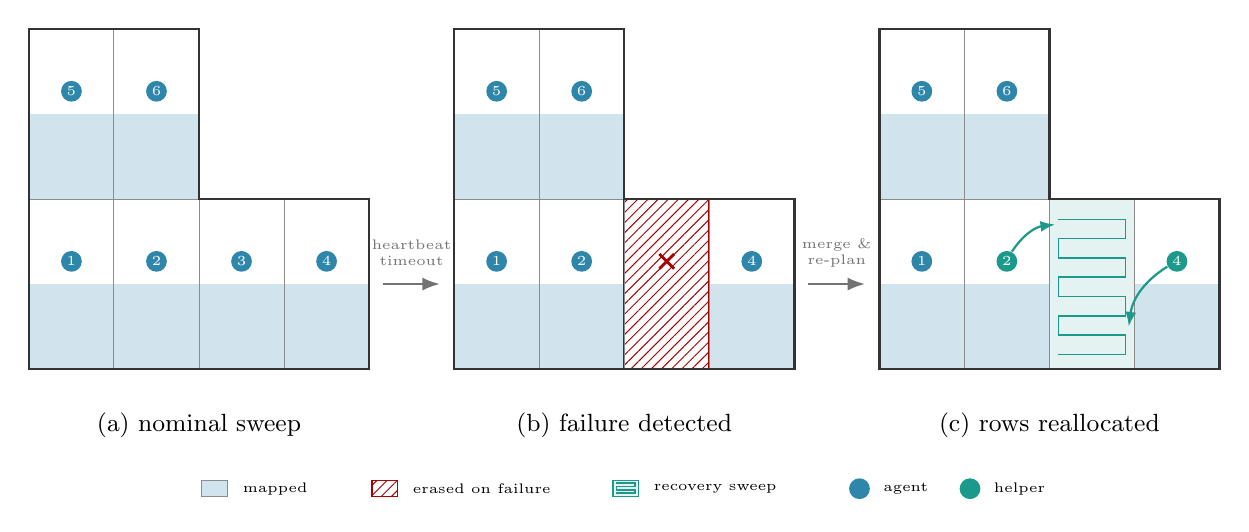
\begin{tikzpicture}[
            scale=0.72,
            every node/.style={font=\scriptsize},
            edge/.style={draw=black!80, line width=0.9pt},
            cut/.style={draw=black!45, line width=0.35pt},
            mapped/.style={fill=layerhigh!22},
            drone/.style={circle, fill=layerhigh, text=white, inner sep=0pt,
                    minimum size=7.5pt, font=\tiny},
            helperdrone/.style={circle, fill=layersim, text=white, inner sep=0pt,
                    minimum size=7.5pt, font=\tiny},
            plab/.style={font=\small},
            leg/.style={font=\tiny}
        ]

        \def\Lregion{(0,0) -- (6,0) -- (6,3) -- (3,3) -- (3,6) -- (0,6) -- cycle}
        \def\Lcuts{%
            \draw[cut] (1.5,0) -- (1.5,6);
            \draw[cut] (3,0) -- (3,3);
            \draw[cut] (4.5,0) -- (4.5,3);
            \draw[cut] (0,3) -- (3,3);
        }

        % =============== (a) sapuan nominal ===============
        \begin{scope}[shift={(0,0)}]
            \fill[mapped] (0,0) rectangle (6,1.5);
            \fill[mapped] (0,3) rectangle (3,4.5);
            \Lcuts
            \draw[edge] \Lregion;
            \node[drone] at (0.75,1.9) {1};
            \node[drone] at (2.25,1.9) {2};
            \node[drone] at (3.75,1.9) {3};
            \node[drone] at (5.25,1.9) {4};
            \node[drone] at (0.75,4.9) {5};
            \node[drone] at (2.25,4.9) {6};
            \node[plab] at (3,-1.0) {(a) nominal sweep};
        \end{scope}

        % =============== (b) agen 3 gugur ===============
        \begin{scope}[shift={(7.5,0)}]
            \fill[mapped] (0,0)   rectangle (3,1.5);
            \fill[mapped] (4.5,0) rectangle (6,1.5);
            \fill[mapped] (0,3)   rectangle (3,4.5);
            \fill[pattern={Lines[angle=45,distance=2.6pt,line width=0.35pt]},
                pattern color=red!65!black] (3,0) rectangle (4.5,3);
            \draw[red!65!black, line width=0.9pt] (3,0) rectangle (4.5,3);
            \Lcuts
            \draw[edge] \Lregion;
            \node[drone] at (0.75,1.9) {1};
            \node[drone] at (2.25,1.9) {2};
            \node[drone] at (5.25,1.9) {4};
            \node[drone] at (0.75,4.9) {5};
            \node[drone] at (2.25,4.9) {6};
            % penanda agen gugur
            \draw[red!65!black, line width=1.0pt] (3.62,1.77) -- (3.88,2.03);
            \draw[red!65!black, line width=1.0pt] (3.62,2.03) -- (3.88,1.77);
            \node[plab] at (3,-1.0) {(b) failure detected};
        \end{scope}

        % =============== (c) baris dialokasikan ulang ===============
        \begin{scope}[shift={(15.0,0)}]
            \fill[mapped] (0,0)   rectangle (3,1.5);
            \fill[mapped] (4.5,0) rectangle (6,1.5);
            \fill[mapped] (0,3)   rectangle (3,4.5);
            \fill[layersim!12] (3,0) rectangle (4.5,3);
            % boustrophedon baru: SATU lintasan menyambung, menutupi sel penuh
            \draw[layersim, line width=0.55pt]
            (3.16,0.26) -- (4.34,0.26) -- (4.34,0.60) -- (3.16,0.60) --
            (3.16,0.94) -- (4.34,0.94) -- (4.34,1.28) -- (3.16,1.28) --
            (3.16,1.62) -- (4.34,1.62) -- (4.34,1.96) -- (3.16,1.96) --
            (3.16,2.30) -- (4.34,2.30) -- (4.34,2.64) -- (3.16,2.64);
            \Lcuts
            \draw[edge] \Lregion;
            \node[drone] at (0.75,1.9) {1};
            \node[helperdrone] (hb) at (2.25,1.9) {2};
            \node[helperdrone] (hd) at (5.25,1.9) {4};
            \node[drone] at (0.75,4.9) {5};
            \node[drone] at (2.25,4.9) {6};
            \draw[-{Latex[scale=0.8]}, layersim, line width=0.8pt]
            (hb) to[bend left=25] (3.10,2.55);
            \draw[-{Latex[scale=0.8]}, layersim, line width=0.8pt]
            (hd) to[bend right=25] (4.40,0.75);
            \node[plab] at (3,-1.0) {(c) rows reallocated};
        \end{scope}

        % =============== panah alur antar-panel ===============
        % Tanpa ini ketiga panel terbaca sebagai tiga gambar terpisah, bukan
        % satu urutan sebab-akibat. Diletakkan di celah antar-panel.
        \draw[-{Latex[scale=0.9]}, black!55, line width=0.9pt] (6.25,1.5) -- (7.25,1.5);
        \node[font=\tiny, text=black!55, align=center] at (6.75,2.05)
        {heartbeat\\timeout};

        \draw[-{Latex[scale=0.9]}, black!55, line width=0.9pt] (13.75,1.5) -- (14.75,1.5);
        \node[font=\tiny, text=black!55, align=center] at (14.25,2.05)
        {merge \&\\re-plan};

        % =============== legenda bersama ===============
        \begin{scope}[shift={(0,-2.15)}]
            \fill[mapped] (3.05,-0.10) rectangle (3.50,0.18);
            \draw[black!45, line width=0.3pt] (3.05,-0.10) rectangle (3.50,0.18);
            \node[leg, anchor=west] at (3.60,0.04) {mapped};

            \fill[pattern={Lines[angle=45,distance=2.6pt,line width=0.35pt]},
                pattern color=red!65!black] (6.05,-0.10) rectangle (6.50,0.18);
            \draw[red!65!black, line width=0.5pt] (6.05,-0.10) rectangle (6.50,0.18);
            \node[leg, anchor=west] at (6.60,0.04) {erased on failure};

            \fill[layersim!12] (10.30,-0.10) rectangle (10.75,0.18);
            \draw[layersim, line width=0.5pt] (10.30,-0.10) rectangle (10.75,0.18);
            \draw[layersim, line width=0.55pt]
            (10.36,-0.04) -- (10.69,-0.04) -- (10.69,0.02) -- (10.36,0.02) --
            (10.36,0.08) -- (10.69,0.08) -- (10.69,0.14) -- (10.36,0.14);
            \node[leg, anchor=west] at (10.85,0.04) {recovery sweep};

            \node[drone] at (14.65,0.04) {\,};
            \node[leg, anchor=west] at (14.90,0.04) {agent};

            \node[helperdrone] at (16.60,0.04) {\,};
            \node[leg, anchor=west] at (16.85,0.04) {helper};
        \end{scope}

    \end{tikzpicture}
    \caption{Fault-tolerant cooperative coverage, drawn schematically. (a) Each agent sweeps
        its own cell and marks the shared occupancy grid as it goes. (b) Agent~3 stops sending
        heartbeats; because the map it had accumulated was carried on that vehicle, the
        coordinator erases the occupancy record over the whole of $V_3$ rather than crediting
        the part already flown, so the entire cell reverts to unobserved. (c) A fresh
        boustrophedon path is generated over $V_{\mathrm{merged}}$, Eq.~\eqref{eq:e9}, and its
        rows are split between a bounded set of surviving neighbours, which resume their own
        cells once the recovery rows are finished.}
    \label{fig:ftcc-concept}
\end{figure}


\headingtwo{Mid-Level Layer: Decentralized Collision Avoidance}

A control barrier function certifies forward invariance of a safe set through a single
inequality on the control input, and pairing it with a quadratic program yields a minimally
invasive safety filter \citt{amesControlBarrierFunction2017}{amesControlBarrierFunctions2019};
the reciprocal multi-agent form is due to Wang \emph{et al.}
\cit{wangSafetyBarrierCertificates2017}. This section instantiates that construction with a
class-$\mathcal{K}$ function derived from the vehicle rather than tuned.

\headingthree{Closed-Loop Plant Identification}

The barrier is built on the identified closed-loop response of the low-level position
controller, so no constant in this layer is hand-tuned. With the reference rule
$\mathbf{x}_{\mathrm{ref}}=\mathbf{x}+T_{\mathrm{lead}}\mathbf{v}_{\mathrm{cmd}}$ and the
outer-loop law of Eq.~\eqref{eq:e32}, the commanded-velocity plant is first order with acceleration
saturation,

\begin{equation}
    \label{eq:e10}
    \dot v=\mathrm{sat}_{\pm a_{\max}}\bigl(k_v\,(v_{\mathrm{cmd}}-v)\bigr),
\end{equation}

\begin{equation}
    \label{eq:e11}
    k_v=g\,K_d,\qquad
    a_{\max}=g\tan\theta_{\max},\qquad
    T_{\mathrm{lead}}=\frac{K_d-k_{\mathrm{ff}}}{K_p},\qquad
    v_c=\frac{a_{\max}}{k_v},
\end{equation}

where $T_{\mathrm{lead}}$ is chosen so that the DC gain from $v_{\mathrm{cmd}}$ to $v$ is
unity and $v_c$ is the speed above which the saturation binds. Integrating Eq.~\eqref{eq:e10} gives the
exact stopping distance from speed $s$,

\begin{equation}
    \label{eq:e12}
    D(s)=
    \begin{cases}
        \dfrac{s^2+v_c^2}{2a_{\max}}, & s>v_c,   \\[8pt]
        \dfrac{s}{k_v},               & s\le v_c.
    \end{cases}
\end{equation}

\headingthree{Actuator-Consistent Class-$\mathcal{K}$ Function}

Let $h$ be the clearance to a constraint surface and $T_d$ the control dead time. The
admissible approach speed is the largest $s$ that can still be brought to rest within $h$,

\begin{equation}
    \label{eq:e13}
    s\,T_d+D(s)\le h
    \;\Longleftrightarrow\;
    s^2+2aT_d\,s+\bigl(v_c^2-2ah\bigr)\le 0 ,
\end{equation}

whose positive root gives the class-$\mathcal{K}$ function

\begin{equation}
    \label{eq:e14}
    \varphi(h)=\max\Bigl(0,\;-aT_d+\sqrt{\max\bigl(0,\;a^2T_d^2+2ah-v_c^2\bigr)}\Bigr).
\end{equation}

Its inverse, the reaction distance required at closing speed $s$, is

\begin{equation}
    \label{eq:e15}
    \varphi^{-1}(s)=\frac{s^2+2aT_d\,s+v_c^2}{2a},
    \qquad
    h_0=\frac{v_c^2-a^2T_d^2}{2a},
\end{equation}

with $h_0$ the largest clearance at which $\varphi=0$ and the vehicle must already be
stopped. Two properties are used downstream: $\varphi$ is monotone increasing and vanishes
for $h\le h_0$, hence a valid class-$\mathcal{K}$ function; and it is Lipschitz with
constant at most $1/T_d$, so the constraint set never tightens faster than $a$ per second,
giving recursive feasibility with respect to the rate limits of Eq.~\eqref{eq:e20}. A linear
$\alpha(h)=\gamma h$ cannot reproduce the flat zero region below $h_0$ and is therefore
inadmissible near $h\to 0$. Figure~\ref{fig:barrier} shows both properties.

% ---------------------------------------------------------------------
% Ilustrasi konsep barrier, tiga panel:
%   (a) anggaran jarak: s*T_d + D(s) <= h  -> asal-usul phi(h)
%   (b) koreksi normal murni: tangensial lolos
%   (c) plot NUMERIK phi(h) pada a=2.5, T_d=0.15, v_c=0.80
% ---------------------------------------------------------------------
\begin{figure}[tbp]
    \centering
    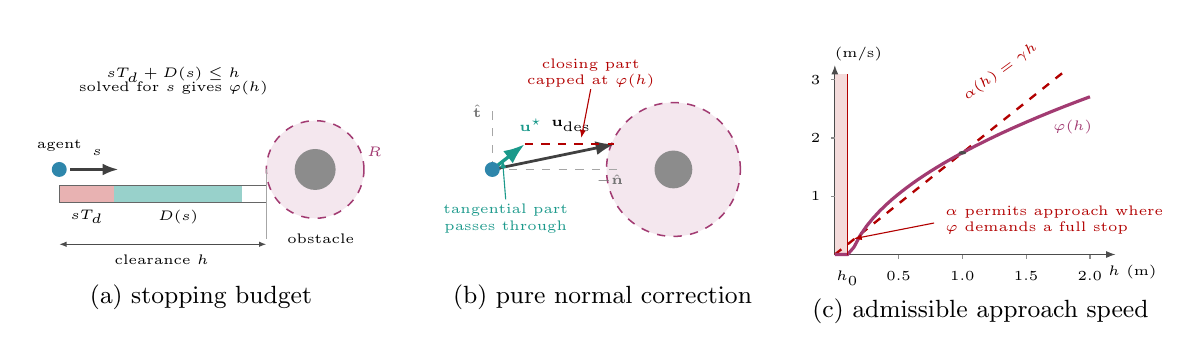
\begin{tikzpicture}[
            every node/.style={font=\scriptsize},
            lbl/.style={font=\tiny},
            panel/.style={font=\small}
        ]

        % ============ (a) anggaran jarak berhenti ============
        \begin{scope}[shift={(0,0)}]
            \fill[layermid!12] (3.55,1.5) circle (0.62);
            \draw[layermid, dashed, line width=0.55pt] (3.55,1.5) circle (0.62);
            \fill[black!45] (3.55,1.5) circle (0.26);
            \node[lbl] at (3.62,0.62) {obstacle};
            \node[lbl, text=layermid] at (4.30,1.72) {$R$};

            \fill[layerhigh] (0.30,1.5) circle (0.095);
            \node[lbl] at (0.30,1.80) {agent};
            \draw[-{Latex[scale=0.8]}, black!75, line width=0.9pt]
            (0.44,1.5) -- (1.05,1.5);
            \node[lbl] at (0.78,1.72) {$s$};

            % pita anggaran: dead time | pengereman | sisa
            \fill[red!70!black!30] (0.30,1.08) rectangle (1.00,1.30);
            \fill[layersim!45]     (1.00,1.08) rectangle (2.62,1.30);
            \draw[black!60, line width=0.4pt] (0.30,1.08) rectangle (2.93,1.30);
            \node[lbl] at (0.65,0.90) {$sT_d$};
            \node[lbl] at (1.81,0.90) {$D(s)$};

            \draw[{Latex[scale=0.55]}-{Latex[scale=0.55]}, black!70, line width=0.4pt]
            (0.30,0.55) -- (2.93,0.55);
            \node[lbl] at (1.60,0.36) {clearance $h$};
            \draw[black!35, line width=0.3pt] (2.93,1.5) -- (2.93,0.62);

            \node[lbl, align=center] at (1.75,2.62)
            {$sT_d+D(s)\le h$\\[-1pt]solved for $s$ gives $\varphi(h)$};

            \node[panel] at (2.1,-0.12) {(a) stopping budget};
        \end{scope}

        % ============ (b) koreksi normal murni ============
        \begin{scope}[shift={(5.35,0)}]
            \fill[layermid!12] (2.75,1.5) circle (0.85);
            \draw[layermid, dashed, line width=0.55pt] (2.75,1.5) circle (0.85);
            \fill[black!45] (2.75,1.5) circle (0.24);

            \draw[black!35, dashed, line width=0.4pt] (0.45,1.5) -- (2.05,1.5);
            \draw[black!35, dashed, line width=0.4pt] (0.45,1.5) -- (0.45,2.30);
            \node[lbl, text=black!55] at (1.94,1.36) {$-\hat{\mathbf{n}}$};
            \node[lbl, text=black!55] at (0.26,2.24) {$\hat{\mathbf{t}}$};

            \draw[-{Latex[scale=0.9]}, black!75, line width=1.0pt]
            (0.45,1.5) -- (2.00,1.82);
            \node[lbl] at (1.45,2.05) {$\mathbf{u}_{\mathrm{des}}$};

            \draw[-{Latex[scale=0.9]}, layersim, line width=1.2pt]
            (0.45,1.5) -- (0.86,1.82);
            \node[lbl, text=layersim] at (0.94,2.06) {$\mathbf{u}^\star$};

            \draw[red!70!black, line width=0.7pt, dashed] (0.86,1.82) -- (2.00,1.82);
            \node[lbl, text=red!70!black, align=center] at (1.70,2.72)
            {closing part\\capped at $\varphi(h)$};
            \draw[-{Latex[scale=0.6]}, red!70!black, line width=0.4pt]
            (1.70,2.52) -- (1.58,1.90);

            \fill[layerhigh] (0.45,1.5) circle (0.095);
            \node[lbl, text=layersim, align=center] at (0.62,0.88)
            {tangential part\\passes through};
            \draw[-{Latex[scale=0.6]}, layersim, line width=0.4pt]
            (0.62,1.12) -- (0.58,1.62);

            \node[panel] at (1.85,-0.12) {(b) pure normal correction};
        \end{scope}

        % ============ (c) phi(h) numerik ============
        \begin{scope}[shift={(10.15,0.42)}]
            \begin{scope}[xscale=1.62, yscale=0.74]
                \fill[red!70!black, opacity=0.14] (0,0) rectangle (0.0999,3.1);
                \draw[-{Latex[scale=0.7]}, black!70] (0,0) -- (2.20,0);
                \draw[-{Latex[scale=0.7]}, black!70] (0,0) -- (0,3.25);
                \foreach \x in {0.5,1.0,1.5,2.0} \draw[black!45] (\x,0) -- (\x,-0.08);
                \foreach \y in {1,2,3} \draw[black!45] (0,\y) -- (-0.03,\y);
                \draw[red!70!black, dashed, line width=0.85pt] (0,0) -- (1.79,3.125);
                \draw[layermid, line width=1.15pt] plot coordinates {
                        (0.000,0.000) (0.050,0.000) (0.100,0.000) (0.150,0.126) (0.200,0.333)
                        (0.250,0.491) (0.300,0.625) (0.350,0.743) (0.400,0.850) (0.450,0.948)
                        (0.500,1.039) (0.550,1.125) (0.600,1.206) (0.650,1.284) (0.700,1.357)
                        (0.750,1.428) (0.800,1.496) (0.850,1.562) (0.900,1.625) (0.950,1.687)
                        (1.000,1.746) (1.100,1.861) (1.200,1.970) (1.300,2.075) (1.400,2.175)
                        (1.500,2.271) (1.600,2.364) (1.700,2.454) (1.800,2.541) (1.900,2.625)
                        (2.000,2.707)};
                \draw[red!70!black, line width=0.45pt] (0.0999,0) -- (0.0999,3.1);
                \fill[black!70] (1.0,1.746) circle (0.030);
            \end{scope}

            % anotasi di luar scope terskala supaya font tidak gepeng
            \foreach \x/\v in {0.81/0.5, 1.62/1.0, 2.43/1.5, 3.24/2.0}
            \node[lbl, below] at (\x,-0.09) {\v};
            \foreach \y/\v in {0.74/1, 1.48/2, 2.22/3}
            \node[lbl, left] at (-0.06,\y) {\v};
            \node[lbl] at (3.78,-0.22) {$h$ (m)};
            \node[lbl] at (0.30,2.55) {(m/s)};
            \node[lbl, text=layermid] at (3.02,1.62) {$\varphi(h)$};
            \node[lbl, text=red!70!black, rotate=36] at (2.10,2.32) {$\alpha(h)=\gamma h$};
            \node[lbl, below] at (0.16,-0.09) {$h_0$};
            \node[lbl, text=red!70!black, align=left, anchor=west] at (1.28,0.44)
            {$\alpha$ permits approach where\\$\varphi$ demands a full stop};
            \draw[-{Latex[scale=0.6]}, red!70!black, line width=0.4pt]
            (1.26,0.40) -- (0.24,0.20);

            \node[panel] at (1.85,-0.72) {(c) admissible approach speed};
        \end{scope}
    \end{tikzpicture}
    \caption{The barrier layer, drawn schematically. (a) The admissible approach speed follows
        from a distance budget: travel during the dead time plus the exact stopping distance
        of Eq.~\eqref{eq:e14} must fit inside the clearance, and solving that inequality for
        $s$ yields $\varphi(h)$. (b) Because the constraint row normal is $-\hat{\mathbf{n}}$,
        the quadratic program caps only the component of the commanded velocity that closes on
        the obstacle; the tangential component passes through unchanged, so the agent skirts
        the obstacle while still making progress. (c) $\varphi(h)$ evaluated at
        $a=2.5$~m/s$^2$, $T_d=0.15$~s, $v_c=0.80$~m/s. Below $h_0$ the admissible speed is
        exactly zero, a flat region no linear $\alpha(h)=\gamma h$ can reproduce: matching the
        two at one clearance (marked) necessarily over-permits nearer in.}
    \label{fig:barrier}
\end{figure}

 The acceleration budget per constraint class $c$ is

\begin{equation}
    \label{eq:e16}
    a_{\mathrm{eff}}^{(c)}=\max\Bigl(0.15\,a_{\max},\;
    \mu_c\,a_{\max}-|a_{\mathrm{obs}}|-|a_{\mathrm{wind}}|\Bigr),
\end{equation}

reserving margin for obstacle acceleration and wind so the row stays satisfiable inside the
rate box.

\headingthree{Constraint Rows}

Every constraint has the form $h=d-R$ with derivative
$\dot h=\hat{\mathbf{n}}^{\!\top}(\mathbf{u}-\mathbf{v}_{\mathrm{obs}})$ and
$\hat{\mathbf{n}}=(\mathbf{p}-\mathbf{o})/\|\mathbf{p}-\mathbf{o}\|$. The CBF condition
$\dot h\ge-\varphi(h)$ becomes a linear row in the commanded velocity $\mathbf{u}$. For
obstacle $k$,

\begin{equation}
    \label{eq:e17}
    -\hat{\mathbf{n}}_k^{\!\top}\mathbf{u}\;\le\;
    \varphi\bigl(h_k,a_{\mathrm{eff}}^{(c)},T_d,v_c\bigr)
    -\hat{\mathbf{n}}_k^{\!\top}\mathbf{v}_k,
    \qquad
    h_k=\|\mathbf{p}-\mathbf{o}_k\|-\bigl(\rho_k+r_d+\delta_c\bigr).
\end{equation}

Because the row normal is $-\hat{\mathbf{n}}_k$, the active-constraint solution is a pure
normal correction, $\mathbf{u}^\star=\mathbf{v}_{\mathrm{nom}}+(\beta-
\hat{\mathbf{n}}^{\!\top}\mathbf{v}_{\mathrm{nom}})\hat{\mathbf{n}}$: the tangential
component passes through unchanged and the agent skirts the obstacle while still making
progress. Inter-agent rows are reciprocal, with responsibility split
$\lambda_{ij}+\lambda_{ji}=1$ weighted by mission state as set out below, and are issued at
two radii so the
soft tier can be released when cells legitimately place agents close together,

\begin{equation}
    \label{eq:e18}
    -\hat{\mathbf{n}}_{ij}^{\!\top}\mathbf{u}_i\le
    \lambda_{ij}\,\varphi\bigl(d_{ij}-R_\bullet\bigr),
    \qquad R_\bullet\in\{R_{\mathrm{hard}},R_{\mathrm{soft}}\}.
\end{equation}

Arena walls and sweep-row stop planes use the outward normal directly,

\begin{equation}
    \label{eq:e19}
    \hat{\mathbf{a}}_w^{\!\top}\mathbf{u}\le\varphi(h_w),
    \quad h_w=\text{signed distance to the plane},
\end{equation}

which replaces the hand-tuned end-of-row feedforward ramp: zero overshoot follows from the
same theorem rather than from a tuned constant. Speed and rate limits are inscribed regular
$n$-gons, guaranteed never to overstate the true disc,

\begin{equation}
    \label{eq:e20}
    A_\Pi(\mathbf{c},r)=\bigl[\cos\vartheta_l,\ \sin\vartheta_l\bigr]_{l=1}^{n},
    \qquad
    b_{\Pi,l}=r\cos\tfrac{\pi}{n}+A_{\Pi,l}\mathbf{c},
    \qquad \vartheta_l=\tfrac{2\pi l}{n},
\end{equation}

evaluated as $\Pi(\mathbf{0},v_{\max})$ for speed and
$\Pi(\mathbf{u}_{\mathrm{prev}},a_{\max}\Delta t)$ for the rate box.

\headingthree{Quadratic Program and Solver}

Stacking all rows into $A\mathbf{u}\le\mathbf{b}$, each agent solves once per tick

\begin{equation}
    \label{eq:e21}
    \mathbf{u}^\star=\arg\min_{\mathbf{u}\in\mathbb{R}^2}
    \tfrac{1}{2}\|\mathbf{u}-\mathbf{u}_{\mathrm{des}}\|^2
    \quad\text{s.t.}\quad A\mathbf{u}\le\mathbf{b},
\end{equation}

a Euclidean projection onto a polyhedron in $\mathbb{R}^2$. In two dimensions the optimum
lies at $\mathbf{u}_{\mathrm{des}}$ when feasible, on a single constraint line, or at the
intersection of a pair, so the complete KKT candidate set

\begin{equation}
    \label{eq:e22}
    \mathcal{U}=\{\mathbf{u}_{\mathrm{des}}\}\cup
    \Bigl\{\mathbf{u}_{\mathrm{des}}-\tfrac{A_l\mathbf{u}_{\mathrm{des}}-b_l}{\|A_l\|^2}A_l^{\!\top}\Bigr\}_{l=1}^{m}
    \cup\Bigl\{\mathbf{u}: A_l\mathbf{u}=b_l,\ A_{l'}\mathbf{u}=b_{l'}\Bigr\}_{l<l'},
\end{equation}

of $1+m+\binom{m}{2}$ points is enumerated, filtered for feasibility, and minimised over.
The result is exact rather than iterative, with no convergence tolerance and no silent
failure. All agents are solved from a single swarm snapshot, which is what makes the
reciprocal split exact.

Each agent carries a manoeuvring willingness $w_i$ fixed by its mission state, and a pair
splits the avoidance burden in proportion to it,

\begin{equation}
    \lambda_{ij}=\frac{w_i}{w_i+w_j},
    \qquad\text{giving}\qquad
    \lambda_{ij}+\lambda_{ji}=1\ \ \text{exactly},
    \label{eq:lambda}
\end{equation}

so summing the two agents' rows recovers the joint condition $\dot h\ge-\varphi(h)$ with no
communication or negotiation. The weights encode who gives way: an agent sweeping a row or
holding its start yaw takes $w=0.25$ and is protected, keeping its mapped line straight; an
agent pausing at a row end takes $w=0.50$; an agent in transit, stepping between rows, or
returning to its centroid takes $w=1.00$; and an agent already finished or waiting for the
swarm takes $w=1.50$ and yields to everyone.

Feasibility is not assumed. Constraint classes are partitioned in advance into \emph{hard}
(static obstacles, moving obstacles, the minimum inter-agent radius), \emph{soft} (arena
walls, the comfortable inter-agent radius, sweep-row stop planes), and \emph{kinematic} (the
speed and rate boxes), and the solver descends a fixed ladder:

\begin{enumerate}[nosep,leftmargin=*,topsep=4pt]
    \item[\textbf{Tier 0.}] Every row is satisfied and the projection of
          Eq.~\eqref{eq:e21} is returned unchanged. This is the normal operating point.
    \item[\textbf{Tier 1.}] Soft classes are released one at a time in the fixed order
          walls, comfortable radius, stop planes, stopping at the first release that
          restores feasibility. Hard classes are never released.
    \item[\textbf{Tier 2.}] Still infeasible: return the command minimising the worst hard
          row violation while staying inside the kinematic box,
          $\min_{\mathbf{u}}\max_l\,(A_l\mathbf{u}-b_l)$ over the hard rows subject to the
          speed and rate rows. The residual is reported as slack, not hidden.
    \item[\textbf{Tier 3.}] Last resort: decay the previous command,
          $\mathbf{u}=0.9\,\mathbf{u}_{\mathrm{prev}}$, so an unbounded or undefined
          velocity is never returned.
\end{enumerate}

The speed and rate boxes are never dropped at any tier, so no tier can command a velocity
the vehicle cannot produce. Figure~\ref{fig:qp} shows both cases.

% ---------------------------------------------------------------------
% Geometri QP di ruang kecepatan.
% Kotak kinematik digambar sebagai OKTAGON (polygon_sides = 8 di kode),
% bukan lingkaran, supaya cocok dengan Eq. baris poligon.
% Panel (b): dua baris keras berlawanan -> irisan kosong, tangga turun.
% ---------------------------------------------------------------------
\begin{figure}[tbp]
    \centering
    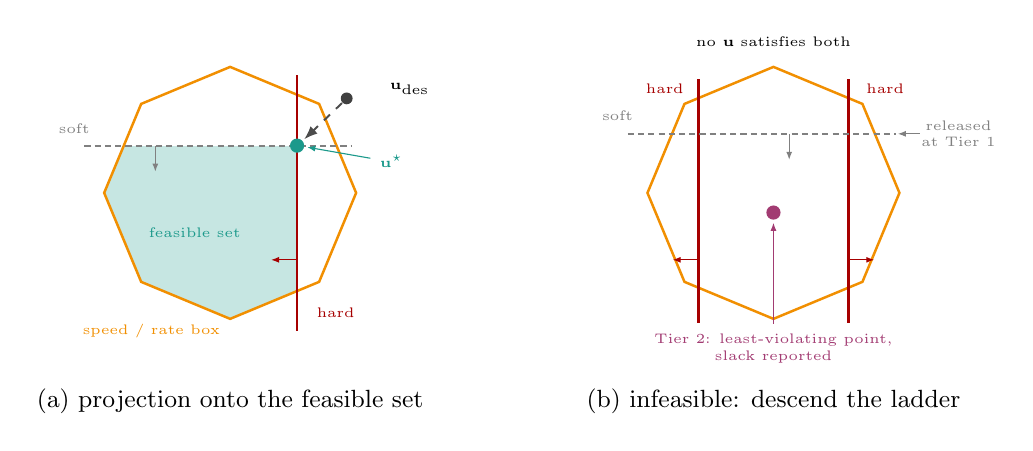
\begin{tikzpicture}[
            every node/.style={font=\scriptsize},
            lbl/.style={font=\tiny},
            plab/.style={font=\small},
            hardl/.style={draw=red!65!black, line width=0.9pt},
            softl/.style={draw=black!50, line width=0.75pt, dash pattern=on 2.2pt off 1.5pt},
            kinl/.style={draw=layerlow, line width=0.9pt},
            lead/.style={-{Latex[scale=0.6]}, line width=0.4pt}
        ]
        % oktagon: pusat (2.0,1.8), circumradius 1.6
        \def\Oct{(3.60,1.80) -- (3.13,2.93) -- (2.00,3.40) -- (0.87,2.93) --
            (0.40,1.80) -- (0.87,0.67) -- (2.00,0.20) -- (3.13,0.67) -- cycle}

        % =============== (a) proyeksi ke himpunan layak ===============
        \begin{scope}
            \begin{scope}
                \clip \Oct;
                \fill[layersim!25] (-1,-1) rectangle (2.85,2.40);
            \end{scope}
            \draw[kinl] \Oct;

            \draw[hardl] (2.85,0.05) -- (2.85,3.30);
            \draw[softl] (0.15,2.40) -- (3.55,2.40);

            % arah sisi layak
            \draw[lead, red!65!black] (2.85,0.95) -- (2.52,0.95);
            \draw[lead, black!50]     (1.05,2.40) -- (1.05,2.07);

            \fill[black!75] (3.48,3.00) circle (0.075);
            \fill[layersim] (2.85,2.40) circle (0.09);
            \draw[-{Latex[scale=0.8]}, black!70, line width=0.7pt, dashed]
            (3.42,2.94) -- (2.94,2.48);

            % label di luar bentuk, dengan penunjuk
            \node[lbl] at (4.28,3.12) {$\mathbf{u}_{\mathrm{des}}$};
            \node[lbl, text=layersim] at (4.05,2.20) {$\mathbf{u}^\star$};
            \draw[lead, layersim] (3.78,2.24) -- (2.98,2.38);
            \node[lbl, text=red!65!black] at (3.34,0.28) {hard};
            \node[lbl, text=black!50] at (0.02,2.62) {soft};
            \node[lbl, text=layerlow] at (1.00,0.05) {speed / rate box};
            \node[lbl, text=layersim] at (1.55,1.30) {feasible set};

            \node[plab] at (2.0,-0.85) {(a) projection onto the feasible set};
        \end{scope}

        % =============== (b) himpunan kosong, tangga turun ===============
        \begin{scope}[shift={(6.9,0)}]
            \draw[kinl] \Oct;

            % dua baris KERAS berlawanan arah -> irisan kosong
            \draw[hardl] (1.05,0.15) -- (1.05,3.25);
            \draw[hardl] (2.95,0.15) -- (2.95,3.25);
            \draw[lead, red!65!black] (1.05,0.95) -- (0.72,0.95);
            \draw[lead, red!65!black] (2.95,0.95) -- (3.28,0.95);

            \draw[softl] (0.15,2.55) -- (3.55,2.55);
            \draw[lead, black!50] (2.20,2.55) -- (2.20,2.22);

            \fill[layermid] (2.00,1.55) circle (0.09);

            \node[lbl, text=red!65!black] at (0.62,3.12) {hard};
            \node[lbl, text=red!65!black] at (3.42,3.12) {hard};
            \node[lbl, text=black!50] at (0.02,2.78) {soft};
            \node[lbl, text=black!50, align=center] at (4.35,2.55)
            {released\\at Tier 1};
            \draw[lead, black!50] (3.86,2.55) -- (3.58,2.55);

            \node[lbl, text=layermid, align=center] at (2.00,-0.18)
            {Tier 2: least-violating point,\\slack reported};
            \draw[lead, layermid] (2.00,0.14) -- (2.00,1.42);

            \node[lbl, align=center] at (2.00,3.72) {no $\mathbf{u}$ satisfies both};

            \node[plab] at (2.0,-0.85) {(b) infeasible: descend the ladder};
        \end{scope}
    \end{tikzpicture}
    \caption{Geometry of the safety filter in velocity space, drawn schematically. (a) Each
        obstacle, neighbour, wall and stop plane contributes one half-plane, and the speed
        and rate limits contribute the inscribed octagon of Eq.~\eqref{eq:e20}; arrows mark
        the admissible side. The command returned is the Euclidean projection of the
        planner's desired velocity onto their intersection, Eq.~\eqref{eq:e21}, computed
        exactly by enumerating the candidate vertices of Eq.~\eqref{eq:e22} --- here the
        projection lands on the corner where two rows are simultaneously active. (b) Two
        opposing hard rows can leave the intersection empty; the ladder then releases soft
        rows in a fixed order and, failing that, returns the least-violating point inside the
        kinematic box with its residual reported as slack. Hard rows and the kinematic box are
        never released, so no tier can command a velocity the vehicle cannot produce.}
    \label{fig:qp}
\end{figure}
 The fraction of ticks resolved above Tier~0 is reported as
$P(\mathrm{tier}>0)$; a value near zero means the ladder is a safety net rather than an
operating mode. Deadlock recovery adds a locked tangential bias to the objective target
only,

\begin{equation}
    \label{eq:e23}
    \mathbf{u}_{\mathrm{des}}\leftarrow\mathbf{u}_{\mathrm{des}}
    +\kappa\,\varsigma_{ik}\,\hat{\mathbf{t}}_{ik},
    \qquad
    \hat{\mathbf{t}}_{ik}=\bigl[-\hat n_{ik,y},\ \hat n_{ik,x}\bigr]^{\!\top},
    \qquad \varsigma_{ik}\in\{-1,+1\},
\end{equation}

with the side $\varsigma_{ik}$ latched per (agent, obstacle) pair to prevent chattering.
Neither $A$ nor $\mathbf{b}$ is ever modified, so liveness is never traded against safety.

\headingtwo{Low-Level Layer: Cascaded PID Robust Control}

\headingthree{Model and Decomposition}

With mass $m$, inertia $\mathrm{diag}(I_x,I_y,I_z)$, thrust $T$, and body torques
$(\tau_x,\tau_y,\tau_z)$, the rigid-body dynamics are \cit{beardSmallUnmannedAircraft2012}

\begin{equation}
    \label{eq:e24}
    m\ddot{\mathbf{p}}=\begin{bmatrix}0\\0\\-mg\end{bmatrix}+R(\phi,\theta,\psi)\begin{bmatrix}0\\0\\T\end{bmatrix},
    \qquad
    I\dot{\boldsymbol{\omega}}+\boldsymbol{\omega}\times I\boldsymbol{\omega}=\boldsymbol{\tau}.
\end{equation}

Linearising about hover ($\phi,\theta\approx 0$, $T\approx mg$) decouples the system into
four double-integrator subsystems, each of the form
$\dot{\mathbf{x}}=A\mathbf{x}+Bu$, $y=C\mathbf{x}$ with

\begin{equation}
    \label{eq:e25}
    A=\begin{bmatrix}0&1\\0&0\end{bmatrix},\qquad
    C=\begin{bmatrix}1&0\end{bmatrix},\qquad
    B\in\Bigl\{\begin{bmatrix}0\\g\end{bmatrix},
    \begin{bmatrix}0\\-g\end{bmatrix},
    \begin{bmatrix}0\\1/I_{y}\end{bmatrix},
    \begin{bmatrix}0\\1/I_{x}\end{bmatrix},
    \begin{bmatrix}0\\1/m\end{bmatrix},
    \begin{bmatrix}0\\1/I_z\end{bmatrix}\Bigr\},
\end{equation}

for the longitudinal outer ($x\!\to\!\theta_{\mathrm{ref}}$), lateral outer
($y\!\to\!\phi_{\mathrm{ref}}$), pitch inner ($\theta\!\to\!\tau_y$), roll inner
($\phi\!\to\!\tau_x$), altitude ($z\!\to\!T$), and yaw ($\psi\!\to\!\tau_z$) loops
respectively. Design weights are listed in Table~\ref{tab:weights}.

\headingthree{Gain Synthesis}

Each loop is augmented with an integrator state,

\begin{equation}
    \label{eq:e26}
    A_a=\begin{bmatrix}A&B\\0&0\end{bmatrix},\quad
    B_a=\begin{bmatrix}0\\I\end{bmatrix},\quad
    Q_a=\mathrm{blkdiag}\bigl(Q,\;0.1\,I\bigr),\quad
    R_a=R\,I .
\end{equation}

PID-LQR solves the continuous algebraic Riccati equation (ARE),

\begin{equation}
    \label{eq:e27}
    A_a^{\!\top}P+PA_a+Q_a-PB_aR_a^{-1}B_a^{\!\top}P=0,
    \qquad K_a=R_a^{-1}B_a^{\!\top}P .
\end{equation}

PID-$H_\infty$ adds an explicit disturbance channel $B_w$ and solves the $H_\infty$ Riccati
equation (HARE) \cit{doyleStateSpaceHinf1989} instead,

\begin{equation}
    \label{eq:e28}
    A_a^{\!\top}P+PA_a+Q_a-P\tilde B\tilde R^{-1}\tilde B^{\!\top}P=0,
    \qquad
    \tilde B=\begin{bmatrix}B_a&B_w\end{bmatrix},\quad
    \tilde R=\begin{bmatrix}R_a&0\\0&-\gamma^2 I\end{bmatrix},
\end{equation}

so that the closed loop satisfies $\|T_{zw}\|_\infty<\gamma$. Both syntheses produce a
state-feedback gain $K_a$ that is mapped onto the PID triple through the structure matrix

\begin{equation}
    \label{eq:e29}
    \Gamma=\begin{bmatrix}
        C^{\!\top} & (CA)^{\!\top} & (CA^2)^{\!\top}\\[2pt]
        0          & (CB)^{\!\top} & (CAB)^{\!\top}
    \end{bmatrix},
    \qquad
    \hat K=\Gamma^{\dagger}K_a^{\!\top}
    =\begin{bmatrix}\hat k_1&\hat k_2&\hat k_3\end{bmatrix}^{\!\top},
\end{equation}

using the Moore--Penrose pseudoinverse, followed by the back-substitution that removes the
algebraic loop introduced by the derivative term,

\begin{equation}
    \label{eq:e30}
    K_d=\hat k_3\bigl(I+CB\,\hat k_3\bigr)^{-1},
    \qquad
    K_i=\bigl(I-K_dCB\bigr)\hat k_1,
    \qquad
    K_p=\bigl(I-K_dCB\bigr)\hat k_2 .
\end{equation}

Both controllers share the identical cascade topology, mixer, and limits, differing only in
whether Eq.~\eqref{eq:e27} or Eq.~\eqref{eq:e28} is solved; any difference in tracking is therefore attributable to gain
synthesis alone.

\headingthree{Selecting the Attenuation Bound}

In Eq.~\eqref{eq:e28} the disturbance enters only through $-\gamma^{-2}B_wB_w^{\!\top}$. As $\gamma$
grows this term shrinks quadratically until it is negligible beside
$B_aR_a^{-1}B_a^{\!\top}$, at which point HARE degenerates into ARE and the $H_\infty$
controller returns gains numerically indistinguishable from LQR. The bound is therefore
placed near its feasibility limit: $\gamma_{\min}$ is located per subsystem by bisection on
the existence of a stabilising solution to Eq.~\eqref{eq:e28}, and the operating value is set to

\begin{equation}
    \label{eq:e31}
    \gamma=1.3\,\gamma_{\min}.
\end{equation}

Table~\ref{tab:gamma} lists both. An earlier iteration of this work used
$\gamma_{\mathrm{out}}=80$, $\gamma_{\mathrm{in}}=64$, which made the disturbance term
$10^3$ to $5\times 10^4$ times smaller than the control term; the two controllers then
agreed to within $2\%$ on every gain and produced near-identical trajectories across a full
mission set.

\headingthree{Control Law and Mixing}

Figure~\ref{fig:cascade} shows the resulting cascade.

% ---------------------------------------------------------------------
% Diagram blok low-level: kaskade PID, sumbu longitudinal sebagai wakil.
% Koordinat ditulis eksplisit (bukan relatif) supaya jalur feedforward dan
% umpan balik tidak saling memotong.
% ---------------------------------------------------------------------
\begin{figure}[tbp]
    \centering
    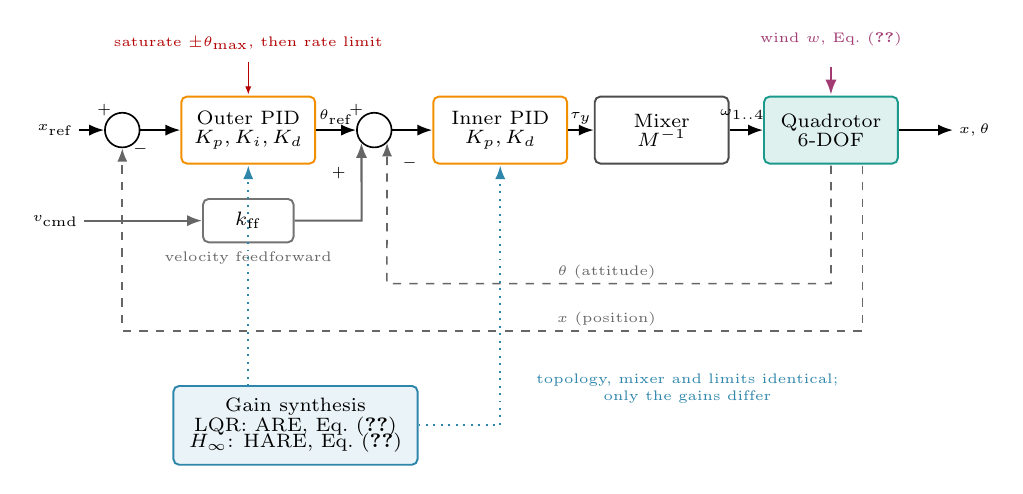
\begin{tikzpicture}[
            every node/.style={font=\scriptsize},
            blk/.style={draw, rounded corners=2pt, line width=0.7pt, align=center,
                    minimum height=0.85cm, minimum width=1.7cm, fill=white, inner sep=2.5pt},
            sum/.style={circle, draw, line width=0.6pt, inner sep=0pt, minimum size=0.44cm},
            sig/.style={-{Latex[scale=0.85]}, line width=0.75pt},
            fb/.style={-{Latex[scale=0.85]}, line width=0.6pt, dashed, black!60},
            lbl/.style={font=\tiny, inner sep=1.8pt},
            note/.style={font=\tiny, align=center, inner sep=1.5pt}
        ]

        % ================= baris utama (y = 0) =================
        \node[lbl]  (ref)   at (-0.10,0) {$x_{\mathrm{ref}}$};
        \node[sum]  (s1)    at ( 0.75,0) {};
        \node[blk, draw=layerlow] (outer) at (2.35,0) {Outer PID\\[-1pt]\scriptsize $K_p,K_i,K_d$};
        \node[sum]  (s2)    at ( 3.95,0) {};
        \node[blk, draw=layerlow] (inner) at (5.55,0) {Inner PID\\[-1pt]\scriptsize $K_p,K_d$};
        \node[blk, draw=black!70] (mix)   at (7.60,0) {Mixer\\[-1pt]\scriptsize $M^{-1}$};
        \node[blk, fill=layersim!14, draw=layersim] (plant) at (9.75,0) {Quadrotor\\[-1pt]\scriptsize 6-DOF};

        \draw[sig] (ref) -- (s1);
        \draw[sig] (s1) -- (outer);
        \draw[sig] (outer) -- node[lbl,above] {$\theta_{\mathrm{ref}}$} (s2);
        \draw[sig] (s2) -- (inner);
        \draw[sig] (inner) -- node[lbl,above] {$\tau_y$} (mix);
        \draw[sig] (mix) -- node[lbl,above,pos=0.38,yshift=1.5pt] {$\omega_{1..4}$} (plant);
        \draw[sig] (plant) -- (11.30,0) node[lbl,right] {$x,\theta$};

        \node[lbl] at (0.52,0.26) {$+$};  \node[lbl] at (0.98,-0.24) {$-$};
        \node[lbl] at (3.72,0.26) {$+$};  \node[lbl] at (4.40,-0.42) {$-$};

        % ================= batas kemiringan =================
        \node[note, text=red!70!black] at (2.35,1.10) {saturate $\pm\theta_{\max}$, then rate limit};
        \draw[-{Latex[scale=0.6]}, red!70!black, line width=0.45pt] (2.35,0.86) -- (2.35,0.45);

        % ================= gangguan angin =================
        \node[note, text=layermid] at (9.75,1.16) {wind $w$, Eq.~\eqref{eq:e36}};
        \draw[sig, layermid] (9.75,0.80) -- (9.75,0.45);

        % ================= feedforward kecepatan (y = -1.15) =================
        \node[blk, minimum width=1.15cm, minimum height=0.55cm, draw=black!55]
        (kff) at (2.35,-1.15) {\scriptsize $k_{\mathrm{ff}}$};
        \node[lbl] (vc) at (-0.10,-1.15) {$v_{\mathrm{cmd}}$};
        \draw[sig, black!60] (vc) -- (kff);
        \draw[sig, black!60] (kff) -- (3.79,-1.15) -- (s2.south west);
        \node[lbl, text=black!60] at (2.35,-1.62) {velocity feedforward};
        \node[lbl] at (3.50,-0.55) {$+$};

        % ================= umpan balik =================
        \draw[fb] (9.75,-0.45) -- (9.75,-1.95) -- (4.11,-1.95) -- (s2.south east);
        \node[lbl, text=black!60] at (6.90,-1.80) {$\theta$ (attitude)};
        \draw[fb] (10.15,-0.45) -- (10.15,-2.55) -- (0.75,-2.55) -- (s1);
        \node[lbl, text=black!60] at (6.90,-2.40) {$x$ (position)};

        % ================= sintesis gain: satu-satunya pembeda =================
        \node[blk, minimum width=3.1cm, minimum height=1.0cm, draw=layerhigh,
            fill=layerhigh!10] (syn) at (2.95,-3.75)
        {Gain synthesis\\[-1pt]\scriptsize LQR: ARE, Eq.~\eqref{eq:e27}\\[-2pt]
        \scriptsize $H_\infty$: HARE, Eq.~\eqref{eq:e28}};
        \draw[-{Latex[scale=0.8]}, layerhigh, line width=0.7pt, dotted]
        (2.35,-3.25) -- (2.35,-1.55) -- (2.35,-0.45);
        \draw[-{Latex[scale=0.8]}, layerhigh, line width=0.7pt, dotted]
        (syn.east) -- (5.55,-3.75) -- (5.55,-0.45);
        \node[note, text=layerhigh, anchor=west] at (5.95,-3.28)
        {topology, mixer and limits identical;\\only the gains differ};

    \end{tikzpicture}
    \caption{Low-level cascade, shown for the longitudinal axis; the lateral, altitude, and
        yaw subsystems have the same structure with the input matrices of
        Eq.~\eqref{eq:e25}. The outer loop maps position error to a reference attitude, which
        is saturated at the tilt limit and rate limited before the inner loop converts
        attitude error to torque; the mixer inverts Eq.~\eqref{eq:e35} to rotor speeds. Both
        controllers under comparison share this topology, mixer, and limits exactly and
        differ only in the shaded synthesis block, so any difference in tracking is
        attributable to gain synthesis alone.}
    \label{fig:cascade}
\end{figure}

With body-frame position errors $e^b_x,e^b_y$ and measured body velocities
$v^b_x,v^b_y$, the outer loops generate reference attitudes with velocity feedforward
$k_{\mathrm{ff}}=0.15$~rad per m/s,

\begin{equation}
    \label{eq:e32}
    \theta_{\mathrm{ref}}=\mathrm{sat}_{\pm\theta_{\max}}\!\Bigl(
    K_p^{x}e^b_x+K_i^{x}\!\!\int\!\! e^b_x
    -K_d^{x}v^b_x+k_{\mathrm{ff}}v^b_{x,\mathrm{cmd}}\Bigr),
    \quad
    \phi_{\mathrm{ref}}=\mathrm{sat}_{\pm\theta_{\max}}\!\Bigl(
    K_p^{y}e^b_y+K_i^{y}\!\!\int\!\! e^b_y
    -K_d^{y}v^b_y-k_{\mathrm{ff}}v^b_{y,\mathrm{cmd}}\Bigr),
\end{equation}

both rate-limited before use. The inner loops, altitude loop, and yaw loop give

\begin{equation}
    \label{eq:e33}
    \tau_y=K_p^{\theta}(\theta_{\mathrm{ref}}-\theta)-K_d^{\theta}q,
    \qquad
    \tau_x=K_p^{\phi}(\phi_{\mathrm{ref}}-\phi)-K_d^{\phi}p,
    \qquad
    \tau_z=K_p^{\psi}e_\psi-K_d^{\psi}r+k_{\mathrm{ff}}^{\psi}\dot\psi_{\mathrm{cmd}},
\end{equation}

\begin{equation}
    \label{eq:e34}
    T=\frac{K_p^{z}e_z+K_i^{z}\!\!\int\!\! e_z+K_d^{z}\dot e_z+mg}{\cos\phi\,\cos\theta},
\end{equation}

where the denominator is the tilt compensation that keeps vertical thrust constant during
manoeuvres. Rotor speeds follow by inverting the mixer, with $d=l\sin 45^\circ$,

\begin{equation}
    \label{eq:e35}
    \begin{bmatrix}T\\\tau_x\\\tau_y\\\tau_z\end{bmatrix}
    =\underbrace{\begin{bmatrix}
            k_f    & k_f   & k_f   & k_f    \\
            -k_fd  & k_fd  & k_fd  & -k_fd  \\
            -k_fd  & k_fd  & -k_fd & k_fd   \\
            -k_m   & -k_m  & k_m   & k_m
        \end{bmatrix}}_{M}
    \begin{bmatrix}\omega_1^2\\\omega_2^2\\\omega_3^2\\\omega_4^2\end{bmatrix},
    \qquad
    \boldsymbol{\omega}=\sqrt{\mathrm{sat}_{[0,\,\omega_{\max}^2]}\bigl(M^{-1}\mathbf{U}\bigr)} .
\end{equation}

\headingthree{Disturbance Model}

Scheme~2 injects a first-order Gauss--Markov gust model approximating Dryden turbulence
\citt{milhdbk1797}{beardSmallUnmannedAircraft2012}. The full Dryden model is a shaping
filter whose spectrum is parameterised by altitude-dependent scale lengths and airspeed;
at the low altitude and low airspeed of a mapping sweep the along-axis component is well
represented by its first-order approximation,

\begin{equation}
    \label{eq:e36}
    w_{k+1}=\alpha_w w_k+\beta_w\varepsilon_k,
    \qquad
    \alpha_w=e^{-\Delta t/\tau_w},
    \qquad
    \beta_w=\sigma_w\sqrt{1-\alpha_w^2},
    \qquad \varepsilon_k\sim\mathcal{N}(0,1),
\end{equation}

with $\sigma_w=2.5$ and $\tau_w=0.5$~s, applied independently per axis. This is the $w$
channel that $B_w$ in Eq.~\eqref{eq:e28} represents.

\begin{table}[tbp]
    \centering
    \begin{minipage}[t]{0.575\textwidth}\centering\footnotesize
        \caption{Design weights per subsystem, Eqs.~\eqref{eq:e25}--\eqref{eq:e26}.}
        \label{tab:weights}
        \begin{tabular}{llcc}
            \toprule
            \textbf{Subsystem / loop} & $\boldsymbol{B}$ & $\boldsymbol{Q}$ & $\boldsymbol{R}$ \\
            \midrule
            Longitudinal $x$, outer   & $[0,\,g]^{\!\top}$      & $\mathrm{diag}(0.05,0.30)$ & $1.00$ \\
            Pitch $\theta$, inner     & $[0,\,1/I_y]^{\!\top}$  & $\mathrm{diag}(2.0,\;0.2)$ & $0.08$ \\
            Lateral $y$, outer        & $[0,\,-g]^{\!\top}$     & $\mathrm{diag}(0.05,0.30)$ & $1.00$ \\
            Roll $\phi$, inner        & $[0,\,1/I_x]^{\!\top}$  & $\mathrm{diag}(2.0,\;0.2)$ & $0.08$ \\
            Altitude $z$              & $[0,\,1/m]^{\!\top}$    & $\mathrm{diag}(1,\;1000)$  & $1.00$ \\
            Yaw $\psi$                & $[0,\,1/I_z]^{\!\top}$  & $\mathrm{diag}(1.0,\;4.0)$ & $4.00$ \\
            \bottomrule
        \end{tabular}
    \end{minipage}\hfill
    \begin{minipage}[t]{0.405\textwidth}\centering\footnotesize
        \caption{$H_\infty$ attenuation bounds. $\gamma_{\min}$ is the feasibility limit of
            Eq.~\eqref{eq:e28}; the operating value is Eq.~\eqref{eq:e31}.}
        \label{tab:gamma}
        \begin{tabular}{lcc}
            \toprule
            \textbf{Subsystem} & $\boldsymbol{\gamma_{\min}}$ & $\boldsymbol{\gamma}$ \\
            \midrule
            Outer position $x$, $y$         & $2.54$ & $3.30$  \\
            Inner attitude $\phi$, $\theta$ & $2.54$ & $3.31$  \\
            Altitude $z$                    & $4.61$ & $6.00$  \\
            Yaw $\psi$                      & $9.02$ & $11.73$ \\
            \bottomrule
        \end{tabular}
    \end{minipage}
\end{table}



\headingtwo{Simulation Setup}

Experiments run in ROS~2 with the Gazebo physics engine, simulating seven quadrotors with
full six-degree-of-freedom rigid-body dynamics, collision geometry, rotor thrust and torque
models, and a first-order motor lag. Parameters are listed in Table~\ref{tab:params}. The
airframe values are those of the 3DR Iris as distributed with PX4, but the PX4 firmware
itself is not in the loop: there is no EKF2 estimator, commander, mixer, or MAVLink
transport, and the controllers under test read vehicle odometry and command rotor speeds
directly through Eq.~\eqref{eq:e35}. This isolates the gain-synthesis comparison, since the PX4
cascade would otherwise dominate the closed-loop response.

\headingthree{Scenarios: A Load Ladder}

The evaluation adds one stressor at a time, so that any change in behaviour is
attributable to the stressor just introduced rather than to an untangleable combination.
Four conditions are flown, each over the same three non-convex regions --- L-shape,
U-shape, plus-shape --- and with both controllers:

\begin{enumerate}[nosep,leftmargin=*,topsep=4pt]
    \item \emph{Nominal}: no disturbance, no obstacles. Establishes the coverage
          capability of the planner on non-convex geometry and provides the reference
          against which every $\Delta$ below is measured.
    \item \emph{Turbulence}: Gauss--Markov gusts, Eq.~\eqref{eq:e36}, no obstacles. Isolates
          the disturbance-rejection contrast between LQR and $H_\infty$.
    \item \emph{Turbulence and obstacles}: as above, plus nine static cylinders placed
          inside each region, which activate the planner-side routing of
          Eqs.~\eqref{eq:e6}--\eqref{eq:e7}. Moving obstacles are excluded; see the
          limitations.
    \item \emph{Turbulence, obstacles, and agent loss}: condition~3 with two agents
          terminated sequentially, the first once coverage reaches $\eta_1=18\%$ and the
          second at $\eta_2=32\%$. The second victim is chosen among the helpers already
          reassigned by the first, so that the compound-polygon merge of Eq.~\eqref{eq:e9}
          and the orphan-row rescue are both exercised rather than only a single clean
          reassignment.
\end{enumerate}

Conditions~3 and~4 differ by the failures alone, which is what makes the coverage loss
attributable to agent loss rather than to the obstacle field. Every mission logs per-agent
telemetry to CSV; all reported values derive from those logs.

\headingthree{Repetitions and Statistical Treatment}

Only the gust sequence is stochastic, and the seed enters nothing else, so the planned
paths are identical across repetitions of a given cell. Conditions~2 and~3 are therefore
flown $N_r=5$ times per region and controller, and condition~4 $N_r=3$ times; condition~1
is deterministic given the initial poses and is flown once, its repetitions serving only to
confirm simulator reproducibility. Results are reported as mean\,$\pm$\,sample standard
deviation. The LQR versus $H_\infty$ contrast is tested on the paired per-(region, seed)
difference with a two-sided Wilcoxon signed-rank test, paired because both controllers see
the identical gust sequence for a given seed. This gives $6+30+30+18=84$ missions, of which
the 12 for conditions~1 and~2 are already available.

\TODO{$N_r$ di atas adalah spesifikasi rancangan. Data yang ADA sekarang baru kondisi 1
    dan 2 pada $N_r=1$; kondisi 3 dan 4 belum dijalankan sama sekali. Sebelum submit:
    jalankan 48 misi sisanya, lalu isi seluruh tabel dengan mean\,$\pm$\,sd dan nilai $p$.
    Kalau waktunya tidak cukup, TURUNKAN klaim $N_r$ di sini dan hapus kolom sd serta uji
    statistiknya --- jangan pernah melaporkan sd dari satu run.}

\begin{table}[tbp]
    \centering
    \begin{minipage}[t]{0.49\textwidth}\centering\footnotesize
        \caption{Airframe and actuator parameters.}
        \label{tab:params}
        \begin{tabular}{llr@{\,}l}
            \toprule
            \textbf{Quantity} & \textbf{Sym.} & \multicolumn{2}{c}{\textbf{Value}} \\
            \midrule
            Mass                  & $m$                & $1.50$    & kg               \\
            Roll/pitch inertia    & $I_x\!=\!I_y$      & $0.0291$  & kg\,m$^2$        \\
            Yaw inertia           & $I_z$              & $0.0552$  & kg\,m$^2$        \\
            Arm length            & $l$                & $0.22$    & m                \\
            Maximum tilt          & $\theta_{\max}$    & $15$      & deg              \\
            Thrust coefficient    & $k_f$              & $8.549$e--6 & N/(rad/s)$^2$  \\
            Torque coefficient    & $k_m$              & $1.368$e--7 & N\,m/(rad/s)$^2$ \\
            Motor time constant   & $\tau_m$           & $0.02$    & s                \\
            Max.\ rotor speed     & $\omega_{\max}$    & $1100$    & rad/s            \\
            Roll/pitch torque cap & $\tau_{rp}^{\max}$ & $0.80$    & N\,m             \\
            Yaw torque cap        & $\tau_{y}^{\max}$  & $0.08$    & N\,m             \\
            \bottomrule
        \end{tabular}
    \end{minipage}\hfill
    \begin{minipage}[t]{0.49\textwidth}\centering\footnotesize
        \caption{Control, planner, and mission parameters.}
        \label{tab:mission}
        \begin{tabular}{llr@{\,}l}
            \toprule
            \textbf{Quantity} & \textbf{Sym.} & \multicolumn{2}{c}{\textbf{Value}} \\
            \midrule
            Attitude feedforward  & $k_{\mathrm{ff}}$    & $0.15$   & rad/(m/s) \\
            Reference lead time   & $T_{\mathrm{lead}}$  & $0.3287$ & s         \\
            Control dead time     & $T_d$                & $0.15$   & s         \\
            Sweep speed           & $v_{\mathrm{sweep}}$ & $1.6$    & m/s       \\
            Command speed cap     & $v_{\max}$           & $3.0$    & m/s       \\
            Sensor radius         & $r_s$                & $0.95$   & m         \\
            Obstacle keep-out     & $R^{\mathrm{ko}}$    & $1.30$   & m         \\
            Voronoi clip margin   & $\delta_c$           & $0.35$   & m         \\
            V2V hard / soft       & $R_{\mathrm{h/s}}$   & $0.70$/$1.20$ & m    \\
            Track confirmation    & $n_{\min}$           & $4$      & hits      \\
            Wind $\sigma_w$, $\tau_w$  & ---             & $2.5$, $0.5$ & N,\,s \\
            Number of agents      & $N$                  & $7$      &           \\
            \bottomrule
        \end{tabular}
    \end{minipage}
\end{table}

\headingthree{Metrics}

Coverage is the fraction of the region occupancy grid observed by at least one agent,

\begin{equation}
    \label{eq:e37}
    \eta=\frac{1}{|\mathcal{G}|}\Bigl|\bigl\{\mathbf{c}\in\mathcal{G}\;\bigm|\;
    \exists\,i,t:\ \|\mathbf{c}-\mathbf{p}_i(t)\|\le r_s\bigr\}\Bigr| .
\end{equation}

For a sweep row through $\mathbf{q}$ with unit direction $\hat{\mathbf{u}}$, the
cross-track and longitudinal lag components of the tracking error are

\begin{equation}
    \label{eq:e38}
    e_{\mathrm{ct}}=\bigl\|(\mathbf{p}-\mathbf{q})-
    \bigl((\mathbf{p}-\mathbf{q})^{\!\top}\hat{\mathbf{u}}\bigr)\hat{\mathbf{u}}\bigr\|,
    \qquad
    e_{\mathrm{lon}}=(\mathbf{p}_{\mathrm{ref}}-\mathbf{p})^{\!\top}\hat{\mathbf{u}},
\end{equation}

the former determining map quality and the latter reflecting the reference-lead policy of
Eq.~\eqref{eq:e11}. Safety and effort are summarised by

\begin{equation}
    \label{eq:e39}
    d_{\min}=\min_{t}\min_{i<j}\|\mathbf{p}_i(t)-\mathbf{p}_j(t)\|,
    \qquad
    J_\tau=\int_0^{T_f}\!\!\|\boldsymbol{\tau}(t)\|_1\,\mathrm{d}t,
    \qquad
    P_{\mathrm{tier}>0}=\frac{1}{N_k}\sum_k \mathbb{1}\bigl[\text{tier}_k>0\bigr].
\end{equation}

For the fault-injection scenario, let $t_f$ be the instant an agent is terminated,
$t_d$ the instant the coordinator declares it dead on heartbeat timeout, and $t_r$ the
instant the first helper begins sweeping a recovery row. The recovery metrics are the
detection latency, the recovery start delay, and the coverage loss against the nominal
mission over the same region,

\begin{equation}
    \Delta t_{\mathrm{det}}=t_d-t_f,
    \qquad
    \Delta t_{\mathrm{rec}}=t_r-t_f,
    \qquad
    \Delta\eta=\eta_{\mathrm{nom}}-\eta_{\mathrm{fault}} ,
\end{equation}

with $\Delta\eta$ expressed in percentage points.

Attitude metrics are computed only over the sweeping phase: samples where the yaw reference
has been stable for at least $1.5$~s and the vehicle exceeds $0.6$~m/s. Whole-mission
percentiles are dominated by the $180^\circ$ pivots at row ends and would misattribute a
normal turn to a disturbance-induced excursion.

% =====================================================================
\headingone{Results and Discussion}

Results follow the load ladder of the previous section. Each subsection adds one stressor
and reports what degrades, what holds, and at what cost.

% =====================================================================
\headingtwo{Coverage Performance on Non-Convex Regions}

Table~\ref{tab:r1} reports the nominal condition and Fig.~\ref{fig:traj}(a) the flown
tracks. \TODO{isi kondisi 1 dari sweep s2\_gamma (pasca perbaikan $\gamma$)}

The coverage figure alone does not establish that the boundary-chain rows are what closes
the tapered corners, since a sweep that simply missed them would still report a high
number. The right-hand columns therefore compare, at planner level and without flying, the
coverage of the path generated by Eq.~\eqref{eq:e5} against a conventional fixed-pitch
sweep over the identical cells. \TODO{jalankan ablasi perencana (offline, tanpa Gazebo)
    dan isi Tabel~\ref{tab:abl}; inilah satu-satunya bukti langsung untuk kontribusi (i)}

\begin{figure}[tbp]
    \centering
    \begin{minipage}[t]{0.48\textwidth}
        \centering
        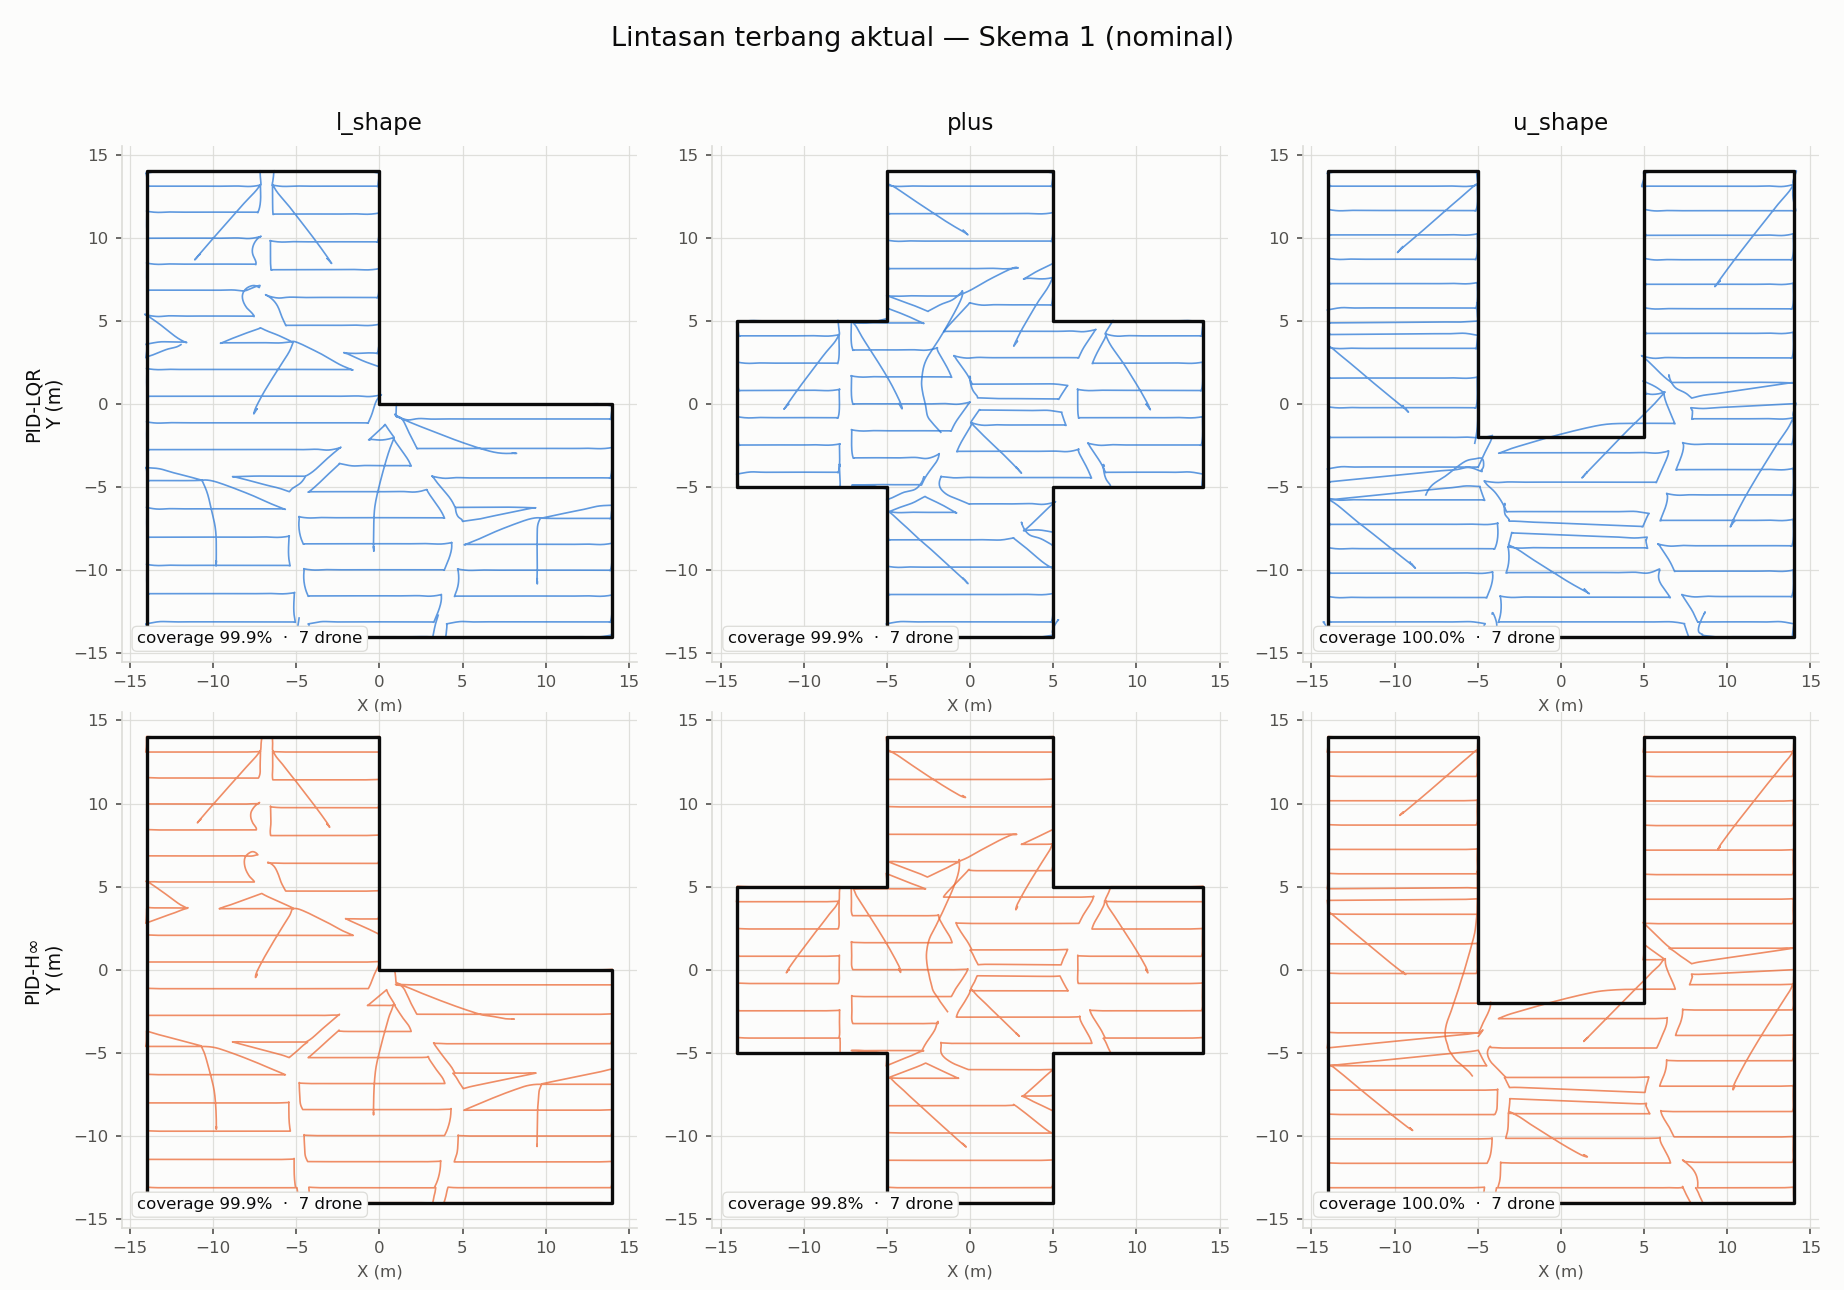
\includegraphics[width=\linewidth]{figures/fig1_trajectories_s1.png}\\
        {\small (a)}
    \end{minipage}\hfill
    \begin{minipage}[t]{0.48\textwidth}
        \centering
        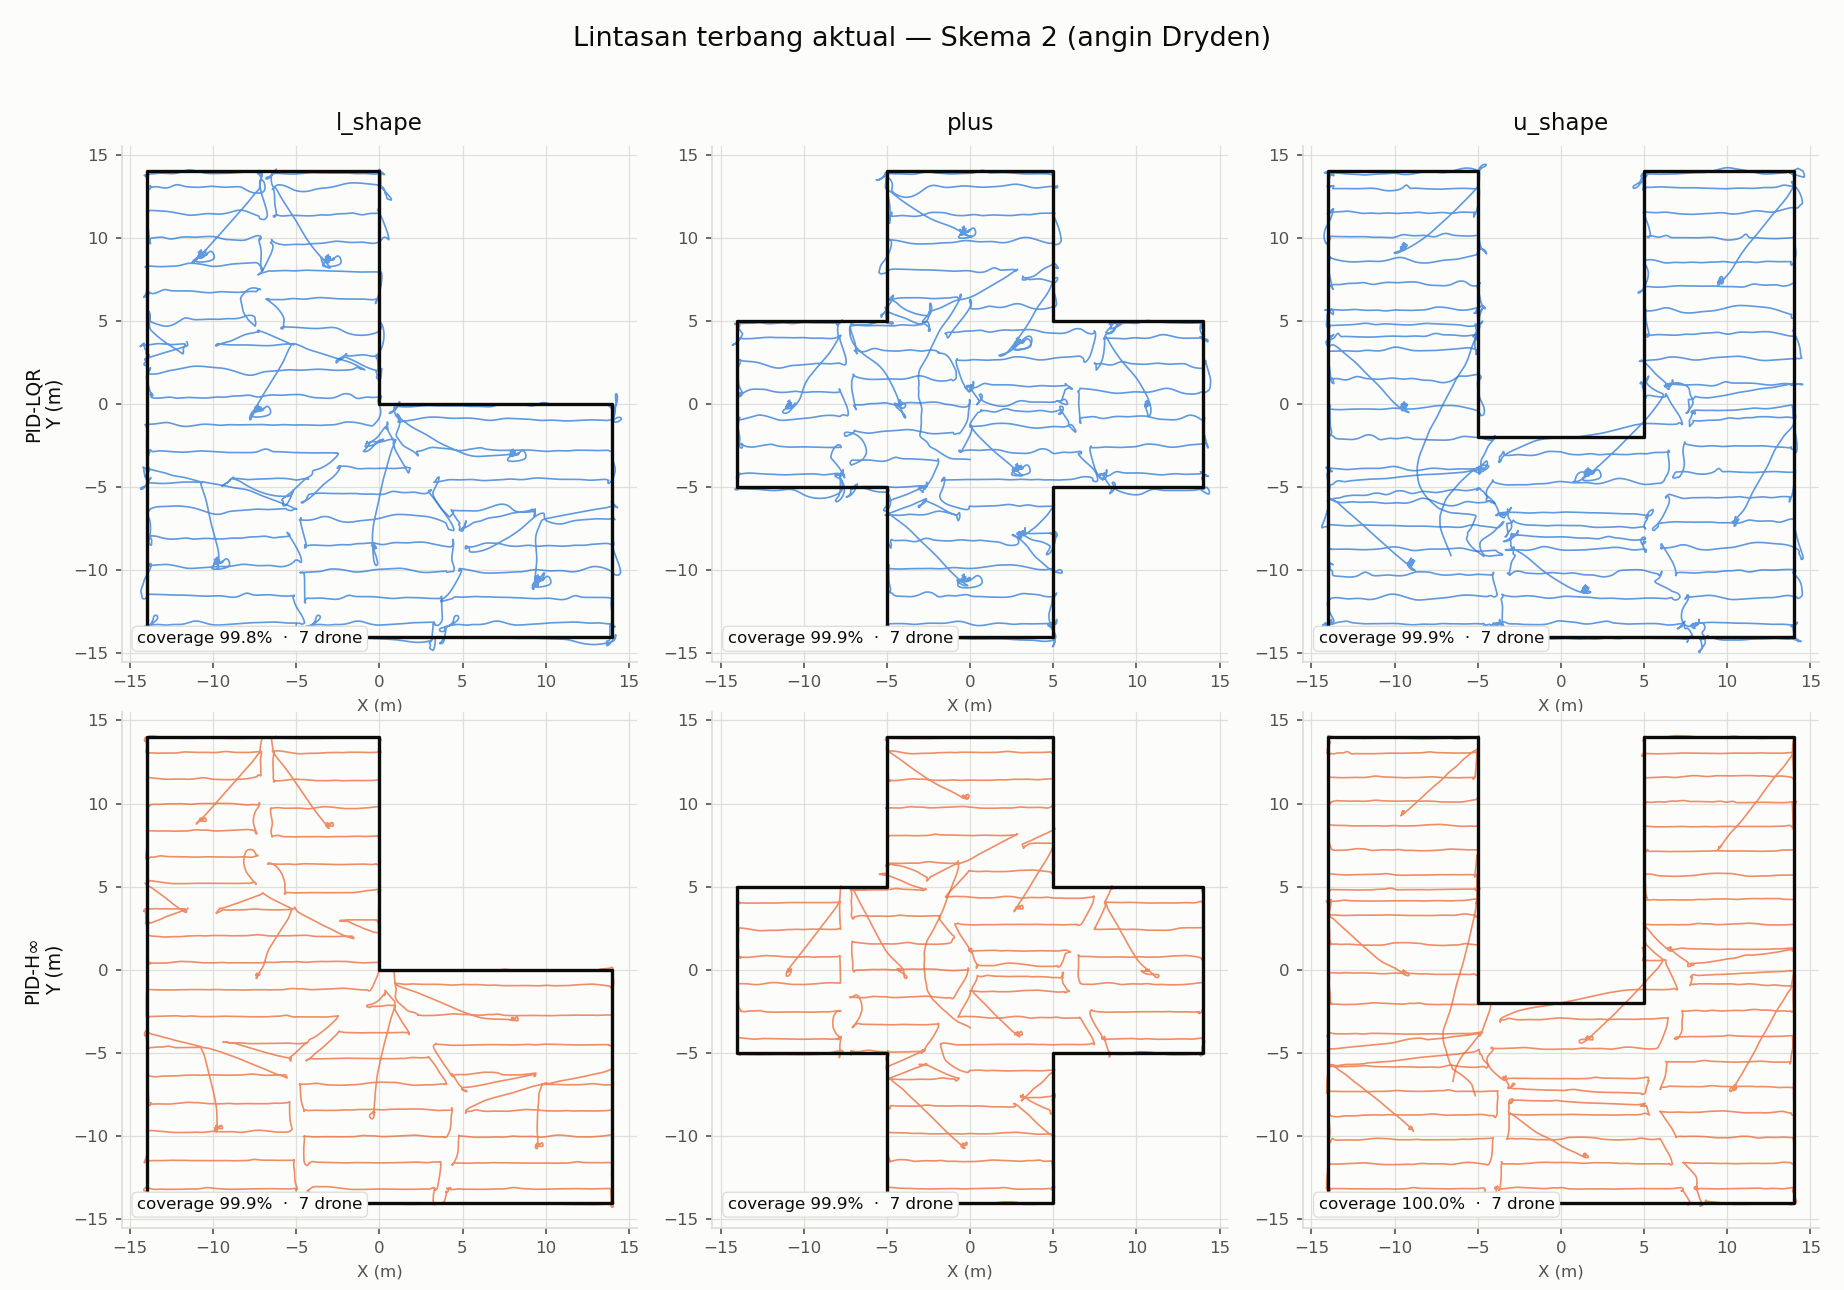
\includegraphics[width=\linewidth]{figures/fig1_trajectories_s2.png}\\
        {\small (b)}
    \end{minipage}
    \caption{Flown trajectories for each non-convex region under (a) the nominal condition
        and (b) turbulence. Cell boundaries from the centroidal Voronoi partition are
        overlaid; the first and last sweep row of each cell follows the cell boundary
        rather than a horizontal line.}
    \label{fig:traj}
\end{figure}

\begin{table}[tbp]
    \centering
    \begin{minipage}[t]{0.56\textwidth}\centering\footnotesize
        \caption{Nominal coverage, flown.}
        \label{tab:r1}
        \begin{tabular}{lcccc}
            \toprule
            \textbf{Region} & $\boldsymbol{\eta}$ \textbf{(\%)} & \textbf{Dur.\ (s)} & \textbf{Path (m)} & $\boldsymbol{d_{\min}}$ \textbf{(m)} \\
            \midrule
            L-shape & \val{--.-} & \val{---} & \val{---} & \val{--.--} \\
            U-shape & \val{--.-} & \val{---} & \val{---} & \val{--.--} \\
            Plus    & \val{--.-} & \val{---} & \val{---} & \val{--.--} \\
            \bottomrule
        \end{tabular}
    \end{minipage}\hfill
    \begin{minipage}[t]{0.42\textwidth}\centering\footnotesize
        \caption{Planner-level ablation: geometric coverage of the planned path, computed
            without simulation.}
        \label{tab:abl}
        \begin{tabular}{lcc}
            \toprule
            \textbf{Region} & \textbf{Fixed pitch} & \textbf{Bnd.\ chain} \\
            \midrule
            L-shape & \val{--.-} & \val{--.-} \\
            U-shape & \val{--.-} & \val{--.-} \\
            Plus    & \val{--.-} & \val{--.-} \\
            \bottomrule
        \end{tabular}
    \end{minipage}
\end{table}

% =====================================================================
\headingtwo{Tracking Performance under Turbulence}

Coverage is expected to survive turbulence because the sweep reference is pinned to the row
line; what degrades is tracking. Table~\ref{tab:r2} reports the contrast.
\TODO{isi dari kondisi 2}

\begin{table}[tbp]
    \centering
    \caption{Tracking accuracy and control effort under turbulence, aggregated over the three regions;
        mean\,$\pm$\,sd over $N_r=5$ seeds. $p$ is the two-sided Wilcoxon signed-rank test
        on the paired per-(region, seed) difference.}
    \label{tab:r2}
    \begin{tabular}{lccccc}
        \toprule
                                  & \multicolumn{2}{c}{\textbf{Nominal}} & \multicolumn{2}{c}{\textbf{Turbulence}} &                  \\
        \cmidrule(lr){2-3}\cmidrule(lr){4-5}
        \textbf{Metric}           & LQR & $H_\infty$ & LQR & $H_\infty$ & $\boldsymbol{p}$ \\
        \midrule
        Cross-track RMS (cm)      & \val{--.--} & \val{--.--} & \val{--.--$\pm$--.--} & \val{--.--$\pm$--.--} & \val{0.0--} \\
        Cross-track p95 (cm)      & \val{--.--} & \val{--.--} & \val{--.--$\pm$--.--} & \val{--.--$\pm$--.--} & \val{0.0--} \\
        Cross-track max (cm)      & \val{--.--} & \val{--.--} & \val{--.--$\pm$--.--} & \val{--.--$\pm$--.--} & \val{0.0--} \\
        Longitudinal lag (cm)     & \val{--.-}  & \val{--.-}  & \val{--.-$\pm$--.-}   & \val{--.-$\pm$--.-}   & \val{0.0--} \\
        Altitude RMS (cm)         & \val{--.--} & \val{--.--} & \val{--.--$\pm$--.--} & \val{--.--$\pm$--.--} & \val{0.0--} \\
        Roll p95, sweeping (deg)  & \val{--.--} & \val{--.--} & \val{--.--$\pm$--.--} & \val{--.--$\pm$--.--} & \val{0.0--} \\
        Pitch p95, sweeping (deg) & \val{--.--} & \val{--.--} & \val{--.--$\pm$--.--} & \val{--.--$\pm$--.--} & \val{0.0--} \\
        \addlinespace
        Torque integral $J_\tau$  & \val{--.--} & \val{--.--} & \val{--.--$\pm$--.--} & \val{--.--$\pm$--.--} & \val{0.0--} \\
        RPM RMS                   & \val{---}   & \val{---}   & \val{---$\pm$-.-}     & \val{---$\pm$-.-}     & \val{0.0--} \\
        \bottomrule
    \end{tabular}
\end{table}

\begin{figure}[tbp]
    \centering
    \fbox{\parbox[c][3.8cm][c]{0.72\textwidth}{\centering
            \TODO{figures/fig5\_crosstrack\_spread.png --- box plot cross-track RMS
                LQR vs $H_\infty$ lintas 5 seed, per region. Inilah yang membenarkan
                pengulangan berseed; tanpa gambar ini angka $\pm$sd tidak terbaca.}}}
    \caption{Spread of cross-track RMS error across gust seeds. Boxes span the inter-quartile
        range over the five seeds; whiskers give the full range.}
    \label{fig:spread}
\end{figure}

Whatever separation appears here follows from the attenuation bound of
Eq.~\eqref{eq:e31}. Table~\ref{tab:degen} makes that dependence concrete: with $\gamma$ set
far above $\gamma_{\min}$, the synthesised $H_\infty$ gains collapse onto the LQR gains, and
the comparison measures nothing. These are properties of the synthesis, obtained without
simulation.

\begin{table}[tbp]
    \centering\footnotesize
    \caption{Degeneration of the $H_\infty$ synthesis at large $\gamma$. Gains are those
        returned by Eq.~\eqref{eq:e28}; the last column is the relative deviation from the
        LQR gain of Eq.~\eqref{eq:e27} for the same subsystem.}
    \label{tab:degen}
    \begin{tabular}{lccc}
        \toprule
        \textbf{Subsystem} & $\boldsymbol{\gamma}$ & $\boldsymbol{K_p}$ & \textbf{Dev.\ from LQR (\%)} \\
        \midrule
        \multicolumn{4}{l}{\emph{Earlier setting, far above $\gamma_{\min}$}} \\
        \quad Outer position & $80$    & \val{--.----} & \val{--.-} \\
        \quad Inner attitude & $64$    & \val{--.----} & \val{--.-} \\
        \quad Yaw            & $64$    & \val{--.----} & \val{--.-} \\
        \addlinespace
        \multicolumn{4}{l}{\emph{Operating setting, $\gamma=1.3\,\gamma_{\min}$}} \\
        \quad Outer position & $3.30$  & \val{--.----} & \val{--.-} \\
        \quad Inner attitude & $3.31$  & \val{--.----} & \val{--.-} \\
        \quad Yaw            & $11.73$ & \val{--.----} & \val{--.-} \\
        \bottomrule
    \end{tabular}
\end{table}

\TODO{isi Tabel~\ref{tab:degen} dengan menjalankan solver pada kedua nilai $\gamma$ dan
    membandingkan gain-nya terhadap LQR --- murni numerik, tanpa Gazebo.}

% =====================================================================
\headingtwo{Coverage and Safety with Static Obstacles}

Nine static cylinders per region activate the planner-side routing and load the barrier
layer while the wind is still acting. Table~\ref{tab:r3} reports the cost of the detours
and the safety margins that survive them, and Fig.~\ref{fig:s4} the resulting tracks.
\TODO{isi dari kondisi 3 (30 misi)}

Two quantities carry the argument. The path-length increase is the price of routing; the
coverage loss $\Delta\eta$ against the nominal condition is what that price buys. Because the keep-out radius
is smaller than the sensing radius, Eq.~\eqref{eq:pitch}, the annulus around each cylinder
is mapped during the detour, so $\Delta\eta$ is expected to stay small even as the path
lengthens. The clearance and feasibility rows test the barrier itself: a
$P(\mathrm{tier}>0)$ that stays near zero means the quadratic program was solvable at its
nominal tier almost everywhere, so the relaxation ladder is a safety net rather than an
operating mode.

Because the map starts empty, the detours in this condition can only be planned once a
cylinder has been found. Table~\ref{tab:percep} reports how well the swarm discovered the
field it was flying through, and Fig.~\ref{fig:discovery} shows the discovery curve against
mission time. \TODO{isi dari log ObstacleMap: bandingkan track terkonfirmasi terhadap
    $\mathcal{O}^{\mathrm{true}}$, catat jarak pertama terdeteksi, dan hitung berapa baris
    sapuan yang sempat direncanakan sebelum rintangannya diketahui.}

\begin{table}[tbp]
    \centering\footnotesize
    \caption{Online obstacle discovery. Nine cylinders are present in each region; the
            planner sees only confirmed tracks.}
        \label{tab:percep}
        \begin{tabular}{lccc}
            \toprule
            \textbf{Quantity} & \textbf{L-shape} & \textbf{U-shape} & \textbf{Plus} \\
            \midrule
            Cylinders confirmed (of 9)      & \val{-}    & \val{-}    & \val{-}    \\
            False tracks confirmed          & \val{-}    & \val{-}    & \val{-}    \\
            Time to first confirmation (s)  & \val{--.-} & \val{--.-} & \val{--.-} \\
            Time to last confirmation (s)   & \val{---}  & \val{---}  & \val{---}  \\
            Detection range, median (m)     & \val{--.-} & \val{--.-} & \val{--.-} \\
            Rows replanned after discovery  & \val{--}   & \val{--}   & \val{--}   \\
            \bottomrule
        \end{tabular}
\end{table}

\begin{figure}[tbp]
    \centering
    \fbox{\parbox[c][3.6cm][c]{0.76\textwidth}{\centering
            \TODO{figures/fig6\_discovery.png --- jumlah silinder terkonfirmasi terhadap
                waktu misi untuk ketiga region, garis putus-putus pada 9 (jumlah sebenarnya),
                dan penanda saat re-plan dipicu}}}
    \caption{Online obstacle discovery against mission time. The dashed line marks the nine
        cylinders actually present; the gap between the curve and that line is the part of
        the field the planner was still unaware of, during which safety rested on the
        barrier layer alone.}
    \label{fig:discovery}
\end{figure}

\begin{table}[tbp]
    \centering
    \caption{Coverage and safety under turbulence with static obstacles; mean\,$\pm$\,sd over $N_r=5$ seeds.
        $\Delta$ columns are measured against the nominal condition of Table~\ref{tab:r1}.}
    \label{tab:r3}
    \begin{tabular}{lcccccc}
        \toprule
                                        & \multicolumn{2}{c}{\textbf{L-shape}} & \multicolumn{2}{c}{\textbf{U-shape}} & \multicolumn{2}{c}{\textbf{Plus}} \\
        \cmidrule(lr){2-3}\cmidrule(lr){4-5}\cmidrule(lr){6-7}
        \textbf{Metric}                 & LQR & $H_\infty$ & LQR & $H_\infty$ & LQR & $H_\infty$ \\
        \midrule
        Final coverage $\eta$ (\%)      & \val{--.-} & \val{--.-} & \val{--.-} & \val{--.-} & \val{--.-} & \val{--.-} \\
        Coverage loss $\Delta\eta$ (pp) & \val{--.-} & \val{--.-} & \val{--.-} & \val{--.-} & \val{--.-} & \val{--.-} \\
        Path length increase (\%)       & \val{--.-} & \val{--.-} & \val{--.-} & \val{--.-} & \val{--.-} & \val{--.-} \\
        Min.\ obstacle clearance (m)    & \val{--.--} & \val{--.--} & \val{--.--} & \val{--.--} & \val{--.--} & \val{--.--} \\
        $d_{\min}$ inter-agent (m)      & \val{--.--} & \val{--.--} & \val{--.--} & \val{--.--} & \val{--.--} & \val{--.--} \\
        $P(\mathrm{tier}>0)$ (\%)       & \val{--.--} & \val{--.--} & \val{--.--} & \val{--.--} & \val{--.--} & \val{--.--} \\
        Collisions                      & \val{--}   & \val{--}   & \val{--}   & \val{--}   & \val{--}   & \val{--}   \\
        \bottomrule
    \end{tabular}
\end{table}

\begin{figure}[tbp]
    \centering
    \fbox{\parbox[c][4.6cm][c]{0.86\textwidth}{\centering
            \TODO{figures/fig3\_scheme4\_tracks.png --- lintasan kondisi 3 dan 4 untuk
                ketiga region dan kedua kontroler, dengan sembilan silinder digambar
                dan titik kegagalan ditandai}}}
    \caption{Flown tracks under turbulence and obstacles. Cylinders are drawn to their
        keep-out radius; crosses mark the two agent failures of condition~4.}
    \label{fig:s4}
\end{figure}

% =====================================================================
\headingtwo{Fault-Tolerant Recovery after Agent Loss}

Condition~4 repeats condition~3 with two sequential failures, so the difference between
Tables~\ref{tab:r4}--\ref{tab:r4b} and Table~\ref{tab:r3} isolates the cost of losing agents from the cost
of the obstacle field. \TODO{isi dari kondisi 4 (18 misi)}

\begin{table}[tbp]
    \centering
    \begin{minipage}[t]{0.49\textwidth}\centering\footnotesize
        \caption{Fault-tolerant recovery: detection and coverage outcome. Mean\,$\pm$\,sd
            over $N_r=3$ seeds; $\Delta\eta$ against condition~3.}
        \label{tab:r4}
        \begin{tabular}{lccc}
            \toprule
            \textbf{Metric} & \textbf{L} & \textbf{U} & \textbf{Plus} \\
            \midrule
            $\Delta t_{\mathrm{det}}$, fail 1 (s) & \val{--.-} & \val{--.-} & \val{--.-} \\
            $\Delta t_{\mathrm{det}}$, fail 2 (s) & \val{--.-} & \val{--.-} & \val{--.-} \\
            $\Delta t_{\mathrm{rec}}$, fail 1 (s) & \val{--.-} & \val{--.-} & \val{--.-} \\
            $\Delta t_{\mathrm{rec}}$, fail 2 (s) & \val{--.-} & \val{--.-} & \val{--.-} \\
            \addlinespace
            Final coverage $\eta$ (\%)            & \val{--.-} & \val{--.-} & \val{--.-} \\
            Coverage loss $\Delta\eta$ (pp)       & \val{--.-} & \val{--.-} & \val{--.-} \\
            Duration increase (\%)                & \val{--.-} & \val{--.-} & \val{--.-} \\
            \bottomrule
        \end{tabular}
    \end{minipage}\hfill
    \begin{minipage}[t]{0.49\textwidth}\centering\footnotesize
        \caption{Fault-tolerant recovery: reallocation load and safety maintained during the
            recovery phase.}
        \label{tab:r4b}
        \begin{tabular}{lccc}
            \toprule
            \textbf{Metric} & \textbf{L} & \textbf{U} & \textbf{Plus} \\
            \midrule
            Recovery rows, fail 1     & \val{--} & \val{--} & \val{--} \\
            Recovery rows, fail 2     & \val{--} & \val{--} & \val{--} \\
            Rows rescued as orphans   & \val{--} & \val{--} & \val{--} \\
            Helper agents allocated   & \val{--} & \val{--} & \val{--} \\
            \addlinespace
            $d_{\min}$, recovery (m)  & \val{--.--} & \val{--.--} & \val{--.--} \\
            Min.\ obstacle clear.\ (m)& \val{--.--} & \val{--.--} & \val{--.--} \\
            Collisions                & \val{--} & \val{--} & \val{--} \\
            \bottomrule
        \end{tabular}
    \end{minipage}
\end{table}

\begin{figure}[tbp]
    \centering
    \fbox{\parbox[c][3.8cm][c]{0.78\textwidth}{\centering
            \TODO{figures/fig4\_load\_ladder.png --- coverage terhadap waktu, tiga kurva
                bertumpuk per region: nominal, turbulensi+rintangan, dan
                +kehilangan agen, dengan penanda vertikal di $t_{f,1}$ dan $t_{f,2}$}}}
    \caption{Coverage against mission time along the load ladder. The vertical gap between
        the curves with and without agent loss at mission end is $\Delta\eta$, the coverage
        attributable to agent loss alone; the vertical lines mark the two failures.}
    \label{fig:ladder}
\end{figure}

The safety rows matter as much as the coverage rows. Reallocation moves helpers into cells
they did not plan for, while the wind is still acting and the cylinders are still present,
which is the most demanding load the barrier layer sees anywhere in this study. Separation
holding through that phase is the strongest available evidence that the class-$\mathcal{K}$
function of Eq.~\eqref{eq:e14} is correctly matched to the vehicle.

% =====================================================================
\headingtwo{Computational Cost of the Safety Filter}

Actuator effort is reported alongside the tracking metrics in Table~\ref{tab:r2}, since it
is the price of that tracking. What remains is computation, which determines whether the
safety filter is admissible at the control rate. Table~\ref{tab:rows} gives the size of the
constraint set actually solved and Table~\ref{tab:cost} the resulting solve time.
\TODO{isi kedua tabel; biaya komputasi dari micro-benchmark solver, bukan dari misi}



\begin{table}[tbp]
    \centering
    \begin{minipage}[t]{0.46\textwidth}\centering\footnotesize
        \caption{Constraint-set size actually solved, sampled over all ticks. Feeds the
            $O(m^2)$ cost of Table~\ref{tab:cost}.}
        \label{tab:rows}
        \begin{tabular}{lcc}
            \toprule
            \textbf{Row class} & \textbf{Median} & \textbf{Max} \\
            \midrule
            Static obstacles     & \val{-}  & \val{-}  \\
            Inter-agent (V2V)    & \val{-}  & \val{-}  \\
            Walls + stop planes  & \val{-}  & \val{-}  \\
            Speed + rate box     & 16       & 16       \\
            \midrule
            Total $m$            & \val{--} & \val{--} \\
            \bottomrule
        \end{tabular}
    \end{minipage}\hfill
    \begin{minipage}[t]{0.50\textwidth}\centering\footnotesize
        \caption{CBF-QP solve time per agent per tick, from a standalone benchmark of the
        solver over representative constraint sets.}
    \label{tab:cost}
    \begin{tabular}{lcc}
        \toprule
        \textbf{Quantity}                              & \textbf{Median} & \textbf{p99} \\
        \midrule
        Constraint rows $m$                            & \val{--}   & \val{--}   \\
        Solve time ($\mu$s)                            & \val{---}  & \val{---}  \\
        Per-tick budget for 7 agents ($\mu$s)          & \val{----} & \val{----} \\
        Fraction of the \val{--}~ms control period (\%) & \val{--.-} & \val{--.-} \\
        \bottomrule
    \end{tabular}
    \end{minipage}
\end{table}

The solver is exact rather than iterative, so the p99 figure is a genuine worst case over
the enumerated candidate set of Eq.~\eqref{eq:e22} and not a convergence tail.
\TODO{setelah terisi, nyatakan margin real-time-nya terhadap periode kendali.}

% =====================================================================
\headingtwo{Comparison with Reported Results}

Re-implementation of the baselines was out of scope, so Table~\ref{tab:baseline} positions
the present results against the figures their authors report. The comparison is indicative,
not controlled: domains, agent counts, and sensing models differ, and only
\cit{breitenmoserVoronoiCoverage2010} and \cit{leeAdaptiveCentroidalVoronoi2024} evaluate
non-convex domains at all. No claim of superiority is made on its basis.

\TODO{isi kolom dari angka yang DILAPORKAN di paper masing-masing, jangan dikira-kira;
    tandai "n/r" untuk yang tidak dilaporkan penulisnya.}

\begin{table}[tbp]
    \centering
    \caption{Indicative positioning against reported results. Entries are the values stated
        by the cited authors under their own conditions; ``n/r'' marks a quantity those
        authors do not report.}
    \label{tab:baseline}
    \begin{tabular}{llcccc}
        \toprule
        \textbf{Work} & \textbf{Domain} & \textbf{Agents} & \textbf{Coverage} & \textbf{Full 6-DOF} & \textbf{Fault tol.} \\
        \midrule
        Cort\'es \emph{et al.} \cit{cortesCoverageControl2004}            & convex     & \val{--} & \val{n/r}  & no  & no  \\
        Breitenmoser \emph{et al.} \cit{breitenmoserVoronoiCoverage2010} & non-convex & \val{--} & \val{--.-} & no  & no  \\
        Lee and Lee \cit{leeAdaptiveCentroidalVoronoi2024}                & non-convex & \val{--} & \val{--.-} & no  & \val{--} \\
        Cao \emph{et al.} \cit{caoDistributedWeightedCoverage2023}        & non-convex & \val{--} & \val{--.-} & no  & no  \\
        \addlinespace
        This work                                                         & non-convex & 7        & \val{--.-} & yes & yes \\
        \bottomrule
    \end{tabular}
\end{table}

% Dinaikkan jadi Heading 1 (tercetak "LIMITATIONS"): batasannya menyangkut
% seluruh studi — model sensor, cakupan skenario, umpan balik ideal — bukan
% hanya bagian Hasil, jadi lebih tepat berdiri sendiri sebelum Conclusion.
\headingone{Limitations}

\emph{State feedback is ideal.} Agents receive ground-truth odometry; there is no estimator
noise, bias, or latency. The absolute tracking errors reported here are therefore a lower
bound for an equivalent flight system.

\emph{Coverage is geometric, not radiometric.} As set out with Eq.~\eqref{eq:pitch},
$\eta$ counts area observed within the sensing radius at the required GSD. It does not
model illumination, motion blur, feature matching, or bundle-adjustment residuals, so a
mission reported here as fully covered is one that satisfies the geometric precondition
for mapping, not one whose reconstructed map has been validated. Closing that gap requires
a photogrammetric pipeline in the loop and is the natural next step for the payload side of
this work.

\emph{Moving obstacles are excluded.} The load ladder stops at static cylinders. The
constraint rows of Eq.~\eqref{eq:e17} already carry the obstacle velocity term, so the
formulation extends to translating obstacles, but the resulting behaviour is not yet stable
enough to report and no moving-obstacle results are claimed.

\emph{Fault tolerance is demonstrated on two sequential losses only.} The scenario
terminates at most two of seven agents; behaviour under larger or simultaneous losses, and
under communication loss without vehicle loss, is untested.

\emph{Baselines are not re-implemented.} Table~\ref{tab:baseline} positions this work
against published figures obtained under different domains, agent counts, and sensing
models. It is not a controlled comparison, and no claim of superiority over those methods
is made on its basis.

\emph{No physical flight.} Ground effect, inter-agent rotor wash, and airframe flexibility
are absent from the model and untested.

% =====================================================================
\headingone{Conclusion}

An end-to-end three-layer architecture for geodetic mapping of non-convex regions by a
quadrotor swarm was presented and evaluated on full six-degree-of-freedom dynamics. The
high-level layer partitions an arbitrary polygon by centroidal Voronoi tessellation,
Eqs.~\eqref{eq:e1}--\eqref{eq:e3}, and sweeps each cell with a boustrophedon path whose extremal rows follow the
cell boundary, Eq.~\eqref{eq:e5}, removing the unswept wedges a fixed-pitch sweep leaves at tapered
corners. The mid-level layer resolves all safety constraints in one quadratic program per
agent per tick, Eq.~\eqref{eq:e21}, whose class-$\mathcal{K}$ function, Eq.~\eqref{eq:e14}, is derived from the
identified closed-loop plant rather than tuned. The low-level layer compares LQR and
$H_\infty$ synthesis, Eqs.~\eqref{eq:e27}--\eqref{eq:e30}, on an identical cascade.

Evaluated along a load ladder that adds one stressor at a time over three non-convex
regions, the swarm held \val{XX.X--XX.X\%} coverage with zero inter-agent collisions at every
rung, and the quadratic program remained feasible at its nominal tier in essentially every
tick. Adding nine obstacles per region lengthened paths by \val{XX\%} while costing only
\val{X.X} percentage points of coverage, because the detour radius stays inside the sensing
footprint. Losing two of seven agents on top of that cost a further \val{X.X} points, with
the first helper sweeping a recovery row \val{XX}~s after the failure and separation
maintained throughout the reallocation. Under Dryden turbulence $H_\infty$ reduced
cross-track RMS error by \val{XX\%} relative to LQR at \val{X.X$\times$} the control effort.
A methodological result of independent interest is that the $H_\infty$ attenuation bound must
be chosen near its feasibility limit, Eq.~\eqref{eq:e31}; at large nominal values the Riccati equation
degenerates and the robust controller silently becomes a disguised LQR.

Future work follows from the limitations: completing the obstacle scenarios, extending
fault tolerance to larger simultaneous losses and to communication loss without vehicle
loss, placing a state estimator in the loop, and carrying the architecture to outdoor flight
and heterogeneous teams.

% =====================================================================
\headingone{Acknowledgments}

% Dukungan CITA ITB HANYA untuk biaya konferensi, bukan pendanaan riset —
% dibedakan eksplisit supaya tidak terbaca sebagai research grant.
The authors thank the Center for Instrumentation Technology and Automation (CITA),
Institut Teknologi Bandung, for supporting the conference registration and publication
fees for this paper. CITA provided no research funding, and had no role in the design of
the study, the simulations, the analysis, or the decision to publish.

% =====================================================================
\headingone{References}

\begingroup
\setlength{\parindent}{0pt}
\renewcommand{\bibsection}{}     % judul sudah dicetak \headingone di atas
\bibliographystyle{aipnum4-1}
\bibliography{references}
\endgroup

\end{document}
